\documentclass[
		master, % type of document: seminar, hausarbeit, bachelor, master, diss
		%english, % remove if you want to write in english
		theotuv, %institution: agwi, ucc, vlba or theotuv
		nomencl, % nomenclature on
		hyperref,
		nolof,
		nolot,
		nolst,
		bibnum
		%twoside % two sided output will be generated
	]{mrcc}
\usepackage{adjustbox}
\usepackage{graphicx}
%\usepackage{listings}
%\usepackage[pdflatex=true]{gastex} % geht erst mit version 2.9, CTAN hat aber nur 2.8 vorrätig

%%%%%%%%%%%%%%%%%%%%%%%%%%%%%%%%%%%%%%%%%%%%%%%%%%%%%%%%%%%%%%%%%%%%%%%%%%%%%%%%%%%%%%%%%%%%%%%%%%%%%%%%%%%
% Miscanallous Options                                                                                    %
%%%%%%%%%%%%%%%%%%%%%%%%%%%%%%%%%%%%%%%%%%%%%%%%%%%%%%%%%%%%%%%%%%%%%%%%%%%%%%%%%%%%%%%%%%%%%%%%%%%%%%%%%%%
\graphicspath{{img/}} % sets Path to figure-folder
%\pgfplotsset{compat=1.6} % pgfplot-fix DOES NOT WORK WITH MACTEX

%%%%%%%%%%%%%%%%%%%%%%%%%%%%%%%%%%%%%%%%%%%%%%%%%%%%%%%%%%%%%%%%%%%%%%%%%%%%%%%%%%%%%%%%%%%%%%%%%%%%%%%%%%%
% Styling etc                                                                                             %
%%%%%%%%%%%%%%%%%%%%%%%%%%%%%%%%%%%%%%%%%%%%%%%%%%%%%%%%%%%%%%%%%%%%%%%%%%%%%%%%%%%%%%%%%%%%%%%%%%%%%%%%%%%
% Based on https://github.com/pads-fhs/LaTeX-Template-Thesis/blob/master/lststyles.tex
\usepackage{listings}
\lstloadlanguages{Java,sh,bash,Haskell,HTML,PHP,XML}
\lstdefinelanguage{console}{
  morekeywords={},
  otherkeywords={warumgehtdasnicht>,\$}
}
\newcommand{\lstsettex}
{ \lstset{
		language=TeX,
		numbers=left,
		numberstyle=\tiny,
		stepnumber=1,
		numbersep=5pt,
		keywordstyle=,
		escapeinside={\%*}{*)},
		tabsize=2,
		captionpos=b,
        lineskip=-2pt,
        breaklines=true,
        language=console,
        breaklines=true,
        commentstyle=\textit\color{green},
        keywordstyle=\bfseries\color{blue},
        basicstyle=\ttfamily,
        stringstyle=\ttfamily,
        showstringspaces=false,
        frame=single,
		morekeywords={hline,begin,documentclass,pgfplotsset,pgfplotstableread,addplot,addlegendentry,textbf,table,label,caption,includegraphics,caption,label,end}
		%,linewidth=.9\textwidth
  }
}
\newcommand{\lstsetconsole}
{ \lstset{%language=sh,
		numbers=left,
		numberstyle=\tiny,
		stepnumber=1,
		numbersep=5pt,
		escapeinside={\%*}{*)},
		tabsize=2,
		captionpos=b,
        lineskip=-2pt,
        breaklines=true,
        language=console,
        breaklines=true,
        commentstyle=\textit\color{green},
        keywordstyle=\bfseries\color{blue},
        basicstyle=\ttfamily,
        stringstyle=\ttfamily,
        showstringspaces=false,
        frame=single
  }
}
\lstdefinelanguage{scalaconsole}{
  morekeywords={},
  otherkeywords={scala>,\|}
}
\newcommand{\lstsetrepl}
{ \lstset{%language=sh,
		numbers=left,
		numberstyle=\tiny,
		stepnumber=1,
		numbersep=5pt,
		escapeinside={\%*}{*)},
		captionpos=b,
        lineskip=-2pt,
        breaklines=true,
        language=scalaconsole,
        breaklines=true,
        commentstyle=\textit\color{green},
        keywordstyle=\bfseries\color{blue},
        basicstyle=\ttfamily,
        stringstyle=\ttfamily,
        showstringspaces=false,
        frame=single,
        tabsize=2
  }
}
\newcommand{\lstsetjava}{
 \lstset{language=Java,
 		numbers=left,
		numberstyle=\tiny,
		stepnumber=1,
		numbersep=5pt,
		escapeinside={\%*}{*)},
		captionpos=b,
        breaklines=true,
        commentstyle=\textit\color{green},
        keywordstyle=\bfseries\color{blue},
        basicstyle=\ttfamily,
        stringstyle=\ttfamily,
        showstringspaces=false,
        frame=single,
        tabsize=2,
        literate=
        %linewidth=\textwidth,captionpos=b
        %numbers=left, stepnumber=5, numbersep=10pt
 }
}
\lstdefinelanguage{scala}{
  morekeywords={abstract,case,catch,class,def,%
    do,else,extends,false,final,finally,%
    for,forSome,if,implicit,import,lazy,match,mixin,%
    new,null,object,override,package,%
    private,protected,requires,return,sealed,%
    super,this,throw,trait,true,try,%
    type,val,var,while,with,yield},
  otherkeywords={_,:,=,=>,<-,<\%,<:,>:,\#,@},
  sensitive=true,
  morecomment=[l]{//},
  morecomment=[n]{/*}{*/},
  morestring=[b]",
  morestring=[b]',
  morestring=[b]"""
}
\newcommand{\lstsetscala}{
 \lstset{language=scala,
 		numbers=left,
		numberstyle=\tiny,
		stepnumber=1,
		numbersep=5pt,
		escapeinside={\%*}{*)},
		captionpos=b,
        breaklines=true,
        commentstyle=\textit\color{green},
        keywordstyle=\bfseries\color{blue},
        basicstyle=\ttfamily,
        stringstyle=\ttfamily,
        showstringspaces=false,
        frame=single,
        tabsize=2
        %%linewidth=\textwidth,captionpos=b
        %numbers=left, stepnumber=5, numbersep=10pt
 }
}
\newcommand{\lstsethtml}{
 \lstset{language=HTML,
 		numbers=left,
		numberstyle=\tiny,
		stepnumber=1,
		numbersep=5pt,
		escapeinside={\%*}{*)},
		captionpos=b,
        breaklines=true,
        commentstyle=\textit\color{green},
        keywordstyle=\bfseries\color{blue},
        basicstyle=\ttfamily,
        stringstyle=\ttfamily,
        showstringspaces=false,
        frame=single,
        tabsize=2
        %%linewidth=\textwidth,captionpos=b
        %numbers=left, stepnumber=5, numbersep=10pt
 }
}
\newcommand{\lstsetphp}{
 \lstset{language=PHP,
 		numbers=left,
		numberstyle=\tiny,
		stepnumber=1,
		numbersep=5pt,
		escapeinside={\%*}{*)},
		captionpos=b,
        breaklines=true,
        commentstyle=\textit\color{green},
        keywordstyle=\bfseries\color{blue},
        basicstyle=\ttfamily,
        stringstyle=\ttfamily,
        showstringspaces=false,
        frame=single,
        tabsize=2
        %%linewidth=\textwidth,captionpos=b
        %numbers=left, stepnumber=5, numbersep=10pt
 }
}
\lstnewenvironment{code}
    {\lstset{}%
      \csname lst@SetFirstLabel\endcsname}
    {\csname lst@SaveFirstLabel\endcsname}
\newcommand{\lstsethaskell}{
    \lstset{
      language=Haskell,
		numbers=left,
		numberstyle=\tiny,
		stepnumber=1,
		numbersep=5pt,
		escapeinside={\%*}{*)},
		captionpos=b,
        commentstyle=\textit\color{green},
        keywordstyle=\bfseries\color{blue},
        basicstyle=\ttfamily,
        stringstyle=\ttfamily,
      showstringspaces=false,
      frame=single,
      flexiblecolumns=false,
      basewidth={0.5em,0.45em},
      literate={+}{{$+$}}1 {/}{{$/$}}1 {*}{{$*$}}1 {=}{{$=$}}1
               {==}{{$==$}}2 %{!=}{{$\not\equiv$}}2
               {>}{{$>$}}1 {<}{{$<$}}1 {\\}{{$\lambda$}}1
               {\\\\}{{\char`\\\char`\\}}1
               {->}{{$\rightarrow$} }2 {>=}{{$\geq$}}2 {<-}{{$\leftarrow$}}2
               {<=}{{$\leq$}}2 {=>}{{$\Rightarrow$} }2
               {\ .}{{$\circ$}}2 {\ .\ }{{$\circ$}}2 {(.)}{({$\circ$})}2
               {>>}{{>>}}2 {>>=}{{>>=}}2
               {|}{{$\mid$}}1
    }
}
\lstdefinelanguage{JavaScript}{
  keywords={typeof, new, true, false, catch,%
    function, return, null, catch, switch, var,%
    if, in, while, do, else, case, break},
  ndkeywords={class, export, boolean, throw, implements, import, this},
  sensitive=false,
  comment=[l]{//},
  morecomment=[s]{/*}{*/},
  morestring=[b]',
  morestring=[b]"
}
\newcommand{\lstsetjavascript}{
  \lstset{
		language=JavaScript,
		numbers=left,
		numberstyle=\tiny,
		stepnumber=1,
		numbersep=5pt,
		escapeinside={\%*}{*)},
		captionpos=b,
		breaklines=true,
        commentstyle=\textit\color{green},
        keywordstyle=\bfseries\color{blue},
        basicstyle=\ttfamily,
        stringstyle=\ttfamily,
		showstringspaces=false,
		frame=single,
		tabsize=2
  }
}
\newcommand{\lstsetxml}{
 \lstset{language=XML,
        breaklines=true,
		numbers=left,
		numberstyle=\tiny,
		stepnumber=1,
		numbersep=5pt,
		escapeinside={\%*}{*)},
		captionpos=b,
        commentstyle=\textit\color{green},
        keywordstyle=\bfseries\color{blue},
        basicstyle=\ttfamily,
        stringstyle=\ttfamily,
        frame=single,
        tabsize=2,
        literate=
        %linewidth=\textwidth,captionpos=b
        %numbers=left, stepnumber=5, numbersep=10pt
 }
}
\lstdefinelanguage{CSharp}{
 morekeywords = {abstract,event,new,struct,as,explicit,%
    null,switch,base,extern,object,this,bool,false,%
    operator,throw,break,finally,out,true,byte,fixed,%
    override,try,case,float,params,typeof,catch,for,%
    private,uint,char,foreach,protected,ulong,checked,%
    goto,public,unchecked,class,if,readonly,unsafe,%
    const,implicit,ref,ushort,continue,in,return,using,%
    decimal,int,sbyte,virtual,default,interface,sealed,%
    volatile,delegate,internal,short,void,do,is,sizeof,%
    while,double,lock,stackalloc,else,long,static,%
    enum,namespace,string,partial},
  morecomment = [l]{//},
  morecomment = [l]{///},
  morecomment = [s]{/*}{*/},
  morestring=[b]",
  sensitive = true
}
\newcommand{\lstsetcsharp}{
 \lstset{language=csharp,
        breaklines=true,
        commentstyle=\textit\color{green},
        keywordstyle=\bfseries\color{blue},
        basicstyle=\ttfamily,
        stringstyle=\ttfamily,
        showstringspaces=false,
        frame=single,
        tabsize=2
        %%linewidth=\textwidth,captionpos=b
        %numbers=left, stepnumber=5, numbersep=10pt
 }
}
\lstdefinelanguage{FSharp}{
  morekeywords={abstract,and,as,assert,base,begin,%
    class,default,delegate,do,done,downcast,downto,%
    elif,else,end,exception,extern,false,finally,for,fun,%
    function,if,in,inherit,inline,interface,internal,lazy,%
    let,match,member,module,mutable,namespace,%
    new,not,null,of,open,or,override,private,public,rec,%
    return,static,struct,then,to,true,try,type,upcast,use,%
    val,void,when,while,with,yield,asr,land,lor,lsl,lsr,lxor,%
    mod,sig,atomic,break,checked,component,const,%
    constraint,constructor,continue,eager,event,external,%
    fixed,functor,global,include,method,mixin,object,%
    parallel,process,protected,pure,sealed,tailcall,trait,virtual,volatile},     
  sensitive=false,
  morecomment=[l][\color{greencomments}]{///},
  morecomment=[l][\color{greencomments}]{//},
  morecomment=[s][\color{greencomments}]{{(*}{*)}},
  morestring=[b]"
}
\newcommand{\lstsetfsharp}{
 \lstset{language=fsharp,
 		numbers=left,
		numberstyle=\tiny,
		stepnumber=1,
		numbersep=5pt,
		escapeinside={\%*}{*)},
		captionpos=b,
        breaklines=true,
        commentstyle=\textit\color{green},
        keywordstyle=\bfseries\color{blue},
        basicstyle=\ttfamily,
        stringstyle=\ttfamily,
        showstringspaces=false,
        frame=single,
        tabsize=2
        %%linewidth=\textwidth,captionpos=b
        %numbers=left, stepnumber=5, numbersep=10pt
 }
}

%%%%%%%%%%%%%%%%%%%%%%%%%%%%%%%%%%%%%%%%%%%%%%%%%%%%%%%%%%%%%%%%%%%%%%%%%%%%%%%%%%%%%%%%%%%%%%%%%%%%%%%%%%%
% Author-related information start here                                                                               %
%%%%%%%%%%%%%%%%%%%%%%%%%%%%%%%%%%%%%%%%%%%%%%%%%%%%%%%%%%%%%%%%%%%%%%%%%%%%%%%%%%%%%%%%%%%%%%%%%%%%%%%%%%%
\author{Anjan Chatterjee}
\title{Towards development of a knowledge model for industrial risk assessments}
\bibfiles{literature}
\supervisor{M.Sc. Emanuel Deisler}
\prof{Prof. Dr.-Ing. habil. Till Mossakowski}
\secondprof{Dr. phil. Fabian Neuhaus}
\abstracten{
\bigskip
\paragraph{}
Industrial risk assessment follows a series of logical steps to identify and examine any potential hazards associated with a particular machinery and its sub-components. The ISO 12100 lists the basic hazard analysis and risk evaluation procedures. It also provides a guideline on the safety of a machinery. Such risk assessment is important to make a decision on the safety of machinery for risks to be reduced where necessary. For a Testing, Inspection and Certification (TIC) industry, within the scope of certification, such kind of risk assessment must be checked and commented on them if necessary. This is done manually, which is expensive and time consuming. Also, the assessments performed in the present day scenario are based on the requirements listed in safety standards. These requirements are sometimes fuzzy and difficult to interpret. The goal of this thesis is towards finding an approach to make faster, safer and more efficient risk assessments. The approach used is towards developing a semantic knowledge model from safety standards and human experts. With the connected infrastructure of industry 4.0 and smart machines, such kind of machine-readable representation of knowledge can help for faster risk assessments. They can provide a more refined interpretation of requirements for risk assessments and also preserve knowledge for quicker re-assessments. The project deals with the safety assessment of a laser cutting machine using a knowledge graph based on ontology. The project lays a foundation towards developing a ground for connected risk assessments by connecting the semantics of safety standard and previous risk assessment.

% With the connected infrastructure of industry 4.0 and smart machines, it would be better if there is a machine readable  is it possible to model the knowledge from standards and domain experts

% Domain knowledge is a valuable asset for every business. In recent times, with the advent of Semantic AI, knowledge elicitation from domain experts and preserving it in a database is an important task. A knowledge model facilitates the preservation of human experiences and have a database of  machine-readable representations of domain specific human expertise. This would lay a foundation for a knowledge graph of industrial products which could have important use cases. For a Testing, Inspection and Certification (TIC) industry, such kind of knowledge graph can bring more refined requirement interpretation for a faster and efficient risk assessment. Also, a validation must be performed to ensure the maximum yield of usable knowledge in that domain. Especially for the TIC industry where safety is concerned, the knowledge model must be validated against the expert human knowledge and then present an inference of the model. The research lies in finding a suitable way for knowledge elicitation from expert and safety standard, structuring it in a knowledge graph based on ontology and finally validating it. Also to find out to which extent the process can be automated. Finally, as an outcome, a productive procedure to model knowledge is expected and a working prototype that can be used for industrial safety and security assessments.
}
\acknowledgments{
\bigskip
\paragraph{}
I would like to express my sincere gratitude to the following individuals and organizations, without whom this masters thesis would not have been possible.

\paragraph{} Firstly, I would like to thank TÜV SÜD Product Service GmbH for providing me with the opportunity to work on this topic and for their constant support throughout the duration of my thesis work. Special thanks to my previous supervisor, M.Sc. Dimitri Harder, for his guidance and valuable insights that helped to shape my research direction. Thanks to my current supervisor M.Sc. Emanuel Deisler for his support throughout my thesis. Also my sincere gratitude to M.Sc. Aranya Sarkar for the constant help alongside.

\paragraph{} Most importantly, I would like to thank Prof. Dr.-Ing. habil. Till Mossakowski, for his support and mentorship throughout my work. His guidance and encouragement have been instrumental in shaping this work. Thanks to Dr. phil. Fabian Neuhaus whose valuable insights were significant towards my research. This work wouldn't have been possible without its acceptance in the Research Group for Theoretical Computer Science, Otto-von-Guericke-University Magdeburg.

\paragraph{} Finally, I would like to thank my Maa and Papa for their unwavering support and encouragement throughout my master studies. Their love and encouragement have kept me motivated and focused on achieving my dreams.
}
\dedication{Meinen Eltern\dots} %only for diss
\birthday{01.01.1980} % only for diss
\placeofbirth{Musterland} % only for diss
\reviewer{Prof. A\\ Prof. B} % only for diss

%%%%%%%%%%%%%%%%%%%%%%%%%%%%%%%%%%%%%%%%%%%%%%%%%%%%%%%%%%%%%%%%%%%%%%%%%%%%%%%%%%%%%%%%%%%%%%%%%%%%%%%%%%%
% Content starts here...                                                                                  %
%%%%%%%%%%%%%%%%%%%%%%%%%%%%%%%%%%%%%%%%%%%%%%%%%%%%%%%%%%%%%%%%%%%%%%%%%%%%%%%%%%%%%%%%%%%%%%%%%%%%%%%%%%%
\begin{document}
	\lstsettex
	% \chapter{MRCC {\LaTeX}-Vorlage}
In diesem Beispieldokument erhalten Sie eine kurze Einf\"uhrung in die Nutzung der Vorlage.

\section{Ben\"otigte Pakete}
Die Vorlage ben\"otigt nutzt diverse Pakete, die in der Regel bei jeder \LaTeX -Distribution vorhanden sind und automatisch eingebunden werden. Da die Vorlage auf KOMA-Script basiert, sollten Sie dieses auf jeden Fall installiert haben (bei Vollinstallationen i.d.R. immer der Fall -- ansonsten nachtr\"aglich laden).

\section{Parameter}
Die Vorlage bietet eine Reihe von Parametern, mit deren Hilfe Sie Einstellungen vornehmen k\"onnen. Die Wichtigste betrifft die Art der von Ihnen angefertigten Arbeit. Diese werden im Anschluss an \verb|\documentclass| angegeben.
\begin{itemize}
	\item \texttt{seminar}: Vorlage f\"ur eine Seminararbeit.
	\item \texttt{hausarbeit}: Vorlage f\"ur eine Hausarbeit.
	\item \texttt{bachelor}: Vorlage f\"ur eine Bachelorarbeit.
	\item \texttt{master}: Vorlage f\"ur eine Masterarbeit.
	\item \texttt{diss}: Vorlage f\"ur eine Dissertation.
\end{itemize}

Weitere Optionen zur Parametrisierung der Vorlage:
\begin{itemize}
	\item \texttt{german}: Vorlage in Deutsch. Wird die Angabe weggelassen, ist die Vorlage englisch. 
	\item \texttt{twoside}: Zweiseitiges Layout.
	\item \texttt{bibnum}: Literaturverweise numerisch statt alphanumerisch.
	\item \texttt{notoc}: Kein Inhaltsverzeichnis.
	\item \texttt{nolof}: Kein Abbildungsverzeichnis.
	\item \texttt{nolot}: Kein Tabellenverzeichnis.
	\item \texttt{nolst}: Kein Quelltext-Verzeichnis.
	\item \texttt{nomencl}: Abk\"urzungsverzeichnis.
	\item \texttt{hyperref}: Referenzen k\"onnen angeklickt werden.
\end{itemize}

\section{Verwendung der Vorlage}
Nachfolgend wird die Verwendung der Vorlage erl\"autert, um Ihnen die Benutzung ein wenig zu vereinfachen\dots

\subsection{Seminararbeit}
Die Vorlage f\"ur Seminararbeiten basiert auf \texttt{scrartcl} aus dem Koma-Script-Paket. Eine Seminararbeit enth\"alt \underline{kein} Inhalts-, Abbildungs-, Tabellen- und Quellcodeverzeichnis. Anzugeben sind \textit{author}, \textit{title}, \textit{supervisor}. Ein Dokument k\"onnte wie in Listing \ref{lst:seminar} aussehen.

\begin{lstlisting}[caption={Beispiel f\"ur eine Seminararbeit}, label={lst:seminar}]
\documentclass[german,seminar]{mrcc}

\author{Max Mustermann}
\title{Meine Seminararbeit}
\supervisor{Matthias Splieth}
\bibfiles{bibfilename}

\begin{document}
	
	% Inhalt hier...

\end{document}
\end{lstlisting}

\subsection{Hausarbeit}
Die Vorlage f\"ur Hausarbeiten basiert ebenfalls auf \texttt{scrartcl} aus dem Koma-Script-Paket, enth\"alt aber -- im Gegensatz zur Vorlage f\"ur Seminararbeiten -- ein Inhaltsverzeichnis, Abbildungsverzeichnis etc.  Anzugeben sind \verb|\author|, \verb|\title|, \verb|\supervisor|, \verb|\bibfiles| sowie sowie \verb|\abstracten| f\"ur eine Zusammenfassung Ihrer Hausarbeit. Ein Dokument k\"onnte wie in Listing \ref{lst:hausarbeit} aussehen.

\begin{lstlisting}[caption={Beispiel f\"ur eine Hausarbeit}, label={lst:hausarbeit}]
\documentclass[german,hausarbeit]{mrcc}

\author{Max Mustermann}
\title{Meine erste Hausarbeit}
\supervisor{Matthias Splieth}
\bibfiles{bibfilename}
\abstracten{A B C D E F G \dots}

\begin{document}
	
	% Inhalt hier...

\end{document}
\end{lstlisting}

\subsection{Bachelor-/Masterarbeit}
Bachelor- und Masterarbeit unterschieden sich durch das Titelblatt und durch die genutzten Verzeichnisse sowie einige Kleinigkeiten am Layout von einer Seminararbeit. Sowohl f\"ur eine Bachelor- als auch eine Masterarbeit sind \verb|\author{...}|, \verb|\title{...}|, \verb|\prof{...}| (betreuender Hochschullehrer), \verb|\secondprof{...}| (Zweitgutachter für Masterarbeiten), \verb|\author{supervisor}| (eigentlicher Betreuer), \verb|\bibfiles{...}|, \verb|\abstracten{...}| anzugeben. Ein Beispiel f\"ur ein Dokument ist Listing \ref{lst:bachma} zu entnehmen.

\begin{lstlisting}[caption={Beispiel f\"ur eine Bachelor-/Masterarbeit}, label={lst:bachma}]
\documentclass[german,master]{mrcc}

\author{Max Mustermann}
\title{Meine Masterarbeit}
\prof{Prof. Dr. Klaus Turowski}
\secondprof{Dr.-Ing. Gamal Kassem}
\supervisor{Matthias Splieth}
\bibfiles{bibfilename}
\abstracten{Kurze englische Zusammenfassung...}
\acknowledgments{Wenn es denn sein muss artig danke sagen...}

\begin{document}
	
	% Inhalt hier...

\end{document}
\end{lstlisting}

\subsection{Dissertation}
Die Dissertation unterschiedet sich hinsichtlich einiger Angaben sowie von Layout von einer Bachelor-/Masterarbeit (vgl. Listing \ref{lst:diss}).

\begin{lstlisting}[caption={Beispiel f\"ur eine Dissertation}, label={lst:diss}]
\documentclass[german,diss]{mrcc}

\author{Max Mustermann}
\title{Meine Dissertation}
\bibfiles{bibfilename}
\abstracten{Kurze englische Zusammenfassung...}
\reviewer{Prof. Dr. Klaus Turowski\\Prof. Dr. Nick Riviera\\Prof. Dr. James Moriaty}
\dedication{Meinen lieben Eltern (oder so)}
\acknowledgments{Bei einer Dissertation darf man auch schon mal "Danke" sagen...}

\begin{document}
	
	% Inhalt hier...

\end{document}
\end{lstlisting}

\subsection{Grafiken und Diagramme}
Das Positionieren von Grafiken in \LaTeX kann nervenaufreibend sein und ist bei weitem nicht so einfach handhabbar wie in Microsoft Word\footnote{Pfui!}. Eine Grafik wird in \LaTeX wie folgt platziert (das Ergebnis ist in Abbildung \ref{fig:fig1} zu sehen \dots):

\begin{lstlisting}[caption={Beispiel f\"ur eine Grafik}]
	\begin{figure}[htbp]
	  \begin{center}
	    
\includegraphics[width=0.2\textwidth]{vlba.pdf}
	    \caption{Ein Bild.}
	    \label{fig:fig1}
	  \end{center}
	\end{figure}
\end{lstlisting}

\begin{figure}[htbp]
  \begin{center}
    
\includegraphics[width=0.2\textwidth]{vlba.pdf}
    \caption{Ein Bild.}
    \label{fig:fig1}
  \end{center}
\end{figure}

Bei den verwendeten Grafiken sollten Sie darauf achten, dass Sie Vektorgrafiken verwenden -- ist einfach schicker und vermeidet \"Uberraschungen beim Drucken!

F\"ur das Positionieren von Grafiken empfiehlt sich aber, sollten dabei Probleme auftreten, das Heranziehen weiterer Quellen. Einen guten Einstieg bietet \url{http://en.wikibooks.org/wiki/LaTeX/Floats,_Figures_and_Captions}.

In \LaTeX lassen k\"onnen zudem mit relativ wenig Aufwand sehr ansprechende Diagramme erstellt werden. Daf\"ur werden in dieser Vorlage die Pakete \verb|tikz| und \verb|pgfplots| verwendet. Zu Beginn konfigurieren Sie die Diagramme mittels \verb|\pgfplotsset{...}| (siehe Listing \ref{lst:tikz}). Am nachfolgenden Beispiel k\"onnen Sie sehen, wie Daten aus zwei CSV-Dateien f\"ur die Erstellung eines Plots genutzt werden:

\pgfplotsset{width=.8\linewidth, height=5cm,every axis/.append style={line width=.5pt},every axis legend/.append style={at={(0.5,1.03)},anchor=south}}
\begin{lstlisting}[caption={Beispiel f\"ur Diagramm mit tikz/pgfplot}, label={lst:tikz}]
	\pgfplotsset{width=.8\linewidth, height=5cm,every axis/.append style={line width=.5pt},every axis legend/.append style={at={(0.5,1.03)},anchor=south}} % irgendwo vor dem Diagramm
	\begin{figure}[!h]
		\centering
			\begin{tikzpicture}
				\begin{axis}[xlabel=Achse 1,ylabel=Achse 2,legend columns=4]
					\pgfplotstableread[col sep=semicolon]{data1.csv}\table
					\addplot[smooth,no markers,green] table[] from {\table};
					\addlegendentry{\textbf{Daten 1}};

					\pgfplotstableread[col sep=semicolon]{data2.csv}\table
					\addplot[smooth,no markers,red] table[] from {\table};
					\addlegendentry{\textbf{Data 2}};
				\end{axis}
			\end{tikzpicture}
			\label{fig:fig2}
			\caption{Ein Diagramm.}
	\end{figure}
\end{lstlisting}

\begin{figure}[!ht]
	\centering
		\begin{tikzpicture}
			\begin{axis}[xlabel=Achse 1,ylabel=Achse 2,legend columns=4]
				\pgfplotstableread[col sep=semicolon]{data1.csv}\table
				\addplot[smooth,no markers,green] table[] from {\table};
				\addlegendentry{\textbf{Daten 1}};

				\pgfplotstableread[col sep=semicolon]{data2.csv}\table
				\addplot[smooth,no markers,red] table[] from {\table};
				\addlegendentry{\textbf{Daten 2}};
			\end{axis}
		\end{tikzpicture}
		\label{fig:fig2}
		\caption{Ein Diagramm.}
\end{figure}

Eine hervorragende Einf\"uhrung zu Diagrammen mit \LaTeX ist unter \url{http://www.bakoma-tex.com/doc/latex/pgfplots/pgfplots.pdf} zu bekommen!

\subsection{Tabellen}
F\"ur Tabellen gelten die gleichen Dinge wie f\"ur Grafiken -- das Positionieren macht nicht immer Spa\ss. Ein Beispiel f\"ur eine Tabelle in \LaTeX wird nachfolgend gegeben. F\"ur eine detailliertere Einf\"uhrung siehe z.B. \url{http://www2.informatik.hu-berlin.de/~piefel/LaTeX-PS/Archive-2004/V03-tab1/}.

\begin{lstlisting}[caption={Beispiel f\"ur eine Tabelle}]
\begin{table}[ht]
	\centering
  \begin{tabular}{ l | c || r }
    \hline
    1 & 2 & 3 \\ \hline
    4 & 5 & 6 \\ \hline
    7 & 8 & 9 \\
    \hline
  \end{tabular}
\end{table}
\end{lstlisting}

Als Ergebnis erh\"alt man dann:

\begin{table}[ht]
	\centering
  \begin{tabular}{ l | c || r }
    \hline
    1 & 2 & 3 \\ \hline
    4 & 5 & 6 \\ \hline
    7 & 8 & 9 \\
    \hline
  \end{tabular}
  \caption{Eine Tabelle}
\end{table}

F\"ur besonders lange Tabellen bietet \LaTeX das Paket \verb|longtable| an. Damit k\"onnen Tabellen auch per Umbruch \"uber eine Seite hinausgehen. Beispiel:
\begin{lstlisting}[caption={Beispiel f\"ur longtable}]
\begin{longtable}{|l|r|c|p{2cm}|}
\hline
	links&rechts&zentriert&parbox\\
\hline
	Kurzer Text.&Kurzer Text.&Kurzer Text.&Kurzer Text.\\
\hline
	Text.&Text.&Text.&Sehr sehr sehr sehr sehr sehr sehr Langer Text, um Umbr\"uche innerhalb einer Zelle zu erzeugen.\\
\hline
	Text.&Text.&Text.&\dots\\
\hline
\end{longtable}
\end{lstlisting}

Das Ergebnis sieht dann wie folgt aus:

\begin{longtable}{|l|r|c|p{2cm}|}
\hline
	links&rechts&zentriert&parbox\\
\hline
	Kurzer Text.&Kurzer Text.&Kurzer Text.&Kurzer Text.\\
\hline
	Text.&Text.&Text.&Sehr sehr sehr sehr sehr sehr langer Text, um Umbr\"uche innerhalb einer Zelle zu erzeugen.\\
\hline
	Text.&Text.&Text.&\dots\\
\hline
\caption{Eine Tabelle mit longtable}
\end{longtable}

\subsection{Listings}
Listings werden in der Vorlage \"uber das Paket \verb|listings| eingebunden. Dieses verf\"ugt bereits \"uber Highlighting-Funktionen f\"ur diverse Sprachen (u.a. C, C++, Java, Python, \LaTeX, \dots) und kann beinahe beliebig angepasst werden. Eine Grundkonfiguration f\"ur die Formatierung von Listings ist f\"ur diese Vorlage bereits vorhanden. F\"ur einzelne Sprachen reicht der Aufruf eines Befehls, um ein Listing entsprechend zu formatieren:

\begin{itemize}
	\item \LaTeX\hfill\verb|\lstsettex|
	\item SH\hfill\verb|\lstsetconsole|
	\item Java\hfill\verb|\lstsetjava|
	\item Scala\hfill\verb|\lstsetscala|
	\item HTML\hfill\verb|\lstsethtml|
	\item PHP\hfill\verb|\lstsetphp|
	\item JavaScript\hfill\verb|\lstsetjavascript|
	\item Haskell\hfill\verb|\lstsethaskell|
	\item XML\hfill\verb|\lstsetxml|
	\item C\#\hfill\verb|\lstsetcsharp|
	\item F\#\hfill\verb|\lstsetfsharp|
\end{itemize}

Vor jedem Listing k\"onnen Sie die Einstellungen, die zu Beginn des Dokuments vorgenommen wurden, durch einen der aufgef\"uhrten Befehle neu setzen.

Um die \"Ubersichtlichkeit im \LaTeX-Dokument zu erh\"ohen kann es sinnvoll sein, das Sie ihre Quelltexte in externen Dateien haben und diese nur in ihr TeX-File einbinden. Dies k\"onnen die durch \verb|\lstinputlisting{path_to_filename.c}| erreichen.

Um Listings mit einer Caption und einem Label zu versehen gen\"ugt es, ein Listing wie folgt zu deklarieren: \verb|\begin{lstlisting}[caption={Beschriftung}, label={label}]|.

\subsection{Literaturverzeichnis}
Das Literaturverzeichnis wird automatisch aus Ihrem BibTeX-File(s) und den daraus zitierten Quellen erzeugt. Zitiert wird mit \verb|\cite{quelle}| bzw. aus B\"uchern mit Angabe der Seitenzahl \verb|\cite[S. 10]{quelle}| (Sie w\"urden ja auch bei einer Aussage, die Sie aus der Bibel \"ubernommen haben, schreiben: siehe Bibel ;)).

Aus \verb|\cite{Addicks2008}| wird dann z. B. ein \cite{Addicks2008} (sofern der BibTeX-Eintrag mit dem Schl\"ussel <Addicks2008> denn auch im BibTeX-File vorhanden ist).

\subsection{Abk\"urzungsverzeichnis}
Das Abk\"urzungsverzeichnis wird mit Hilfe des Pakets \verb|nomencl| erzeugt, sofern der Parameter \texttt|nomencl| beim Dokument angegeben und ein makeindex ausgef\"uhrt wurde. Mit \verb|\nomenclature{<Kurz>}{<Lang>}| l\"asst sich dann eine neue Abk\"urzung einf\"uhren.

\section{Sonstiges}
\subsection{Strukturierung der Arbeit}
Es wird empfohlen, dass Sie Ihre Arbeit in verschiedene Unterdateien aufteilen und diese dann mittels \verb|\input{...}| in der Hauptdatei einbinden. Das erh\"oht nicht nur die \"Ubersichtlichkeit, sondern hilft vor allem bei der Suche nach Fehlern -- die zweifelsohne kommen wird ;)

Beispiel:
\begin{lstlisting}[caption={Beispiel f\"ur das Strukturieren der Arbeit}]
\documentclass[german,master]{mrcc}

\author{Max Mustermann}
\title{Meine Masterarbeit}
\prof{Prof. Dr. Klaus Turowski}
\supervisor{Matthias Splieth}
\bibfiles{bibfilename}
\abstracten{Kurze englische Zusammenfassung...}
\acknowledgments{Wenn es denn sein muss artig danke sagen...}

\begin{document}
	
	\input{chap/kapitel1.tex}
	\input{chap/kapitel2.tex}
	% usw...

\end{document}
\end{lstlisting}

\subsection{Umlaute}
Umlaute f\"uhren in \LaTeX gerne zu Kompatibilit\"atsproblemen, weil Umlaute abh\"anging vom Betriebssystem kodiert werden. Am besten kann das Umgangen werden, wenn Umlaute wie folgt angegeben werden: \verb|"A|, \verb|"O|, \verb|"U|, \verb|"a|, \verb|"o| und \verb|"u|.

\subsection{Makefile}
Der Vorlage liegt ein Makefile bei, mit dem Ihr Dokument kompiliert werden kann. Folgende Optionen stehen zu Verf\"ugung:

\begin{itemize}
	\item \texttt{make}: Kompiliert das Dokument.
	\item \texttt{make clean}: Kompiliert und r\"aumt das Verzeichnis auf.
	\item \texttt{make cleanall}: Kompiliert und r\"aumt noch mehr auf (zus\"atzlich: dvi-, ps-, bmt-Files).
\end{itemize}

Kleine Hinweise dazu:

\begin{itemize}
	\item F\"ur Linux-Nutzer: ein \texttt{make} im Terminal gen\"ugt f\"ur das Kompilieren.
	\item F\"ur Mac-Nutzer: einfach das Makefile \"uber das Terminal ausf\"uhren. Daf\"ur m\"ussen Sie jedoch XCode installieren\footnote{Kostenlos \"uber den AppStore}. In XCode w\"ahlen Sie dann unter \textit{XCode->Preferences->Downloads} die Command Line Tools aus und installieren diese. Anschlie{\ss}end k\"onnen Sie \texttt{make} nutzen.
	\item F\"ur Windows-Nutzer: f\"ur die Nutzung des Makefiles k\"onnen Sie z.B. auf cygwin\footnote{\url{http://www.cygwin.com/}} zur\"uckgreifen.
\end{itemize}
        \listoffigures
	\chapter{Introduction} \label{introduction}

\bigskip\bigskip 

Industrial risk assessment is an essential process for ensuring the safety of workers and minimizing the potential for accidents in industrial settings. In recent years, the increasing need for industrial risk assessment has led to the development of various methods and tools to ensure safety in the workplace. With the increasing complexity of modern industrial systems, it has become more challenging to identify potential hazards and assess the associated risks accurately. One of the most promising techniques is the use of knowledge models. Knowledge modeling is a technique that can help experts and practitioners better understand the complex relationships between various factors that contribute to industrial risks. A knowledge model is a representation of the knowledge and expertise of domain experts in a particular field, captured in a structured format that can be easily accessed and utilized. In the context of industrial risk assessment, a knowledge model can help experts identify potential hazards, assess the associated risks, and design appropriate mitigation strategies. Also a knowledge model can bridge the gap between documented safety standards and an expert's interpretation of the standard in a risk assessment.

\section{Motivation}\label{motivation}

The Testing, Inspection and Certification (TIC) industry is a safety-critical sector where a minor failure could result in some serious damage. For this reason, industrial safety and security assessments are expected to deliver continuously-safe products. With the increasing complexity of modern-day products, more and more effort is required to ensure their safety. For example, to test a machinery, multiple standards need to be referred to test each component of the machine so that the overall product could be certified safe to use. 

\paragraph{} The standards are generally large documents with a huge number of requirements that the product needs to fulfil. These standards describe generalized approaches to identify testing requirements, product requirements, recommendations, hazards and risks. Also some requirements are fuzzy and are difficult to perceive. Therefore, when applying such standards for risk assessments, a significant degree of interpretation might be necessary which usually comes from the knowledge and experience of the engineer responsible for the assessment. 

\paragraph{} Now it becomes an expensive, time-consuming and risky activity to construct a safety checklist for assessment, due to the extensive manual work required. Furthermore, as products evolve, re-assessment and modification are necessary which again needs to repeat the whole risk-assessment procedure. Also with time, the experienced engineers are retiring along with their domain knowledge. This means the tacit knowledge of the domain expert is lost forever. Since knowledge is a valuable asset in every business, no organization can afford to lose it. Particularly, in the case of safety intensive TIC industry, the knowledge gathered over experience would directly impact the time consumed and risk assessed in the safety and security assessments.

\section{Problem Statement and Challenges}\label{problem}
Developing a knowledge model for industrial risk assessment is a complex task that poses several challenges. One of the primary challenges is the heterogeneity of the data used in safety standards. This heterogeneity makes it challenging to integrate data from various sources into a coherent knowledge model. Risk assessments involve multiple standards, each having different formats and structures to specify requirements, hazards, preventive measures, reference standards and other information. These information are not grouped separately but stays mixed as regular textual information. This can make the testing requirements fuzzy and often difficult to understand. Addressing this challenge can make industrial risk assessments faster and efficient.

\paragraph{} Additionally, creating a knowledge model from a safety standard and expert's knowledge can be a complex and time-consuming process. There must be some level of automation in extracting relevant data from regular text. This data must also be formalised for the modeling software used. Performing these tasks manually is not the best solution especially for the enormous text corpus of the safety standards. Therefore, an automated or semi-automated approach must be looked into.

\paragraph{} Another challenge in developing a knowledge model for industrial risk assessment is the need to balance comprehensiveness with usability. A comprehensive knowledge model that covers all possible risks and their associated mitigation strategies can be overwhelming for users and difficult to navigate. On the other hand, a model that is too simplistic may not capture all relevant factors and can lead to inaccurate risk assessments. Therefore, striking the right balance between comprehensiveness and usability is crucial to ensure that the knowledge model is effective in practice. This gives rise to another need to ensure that the knowledge model is adaptable and scalable to accommodate changes. As new standard is introduced, processes are modified, and new risks emerge, the knowledge model must be updated to reflect these changes accurately. 

\paragraph{} Finally, ensuring that the knowledge model is accessible and understandable by human as well as it stays functional for future machine readable applications, is essential to its success. The model must be informative, easy to navigate, and provide actionable insights that can be used to make informed decisions. The effectiveness of the knowledge model depends on the quality and relevance of output it provides. Therefore, it must be validated to prove its relevance. 

\section{Research Question} \label{rq}

A number of research questions are formulated to aim at contributing to the motivation described in Section \ref{motivation} and \ref{problem}

\rqformat{\textbf{RQ 1:} How can industrial safety and security assessments be made faster and efficient?}

This is the central research question and broad in sense. RQ 1 would give rise to further specific research questions. 

As discussed in Section \ref{motivation}, domain knowledge of human experts is important in interpretation of requirements from the standards, which in turn would facilitate risk assessments. Therefore, this knowledge from domain experts as well as knowledge from standards must be preserved for re-use. This brings the following question.

\rqformat{\textbf{RQ 2:} How can knowledge from experts and standards be captured for re-use?}

After capturing knowledge, it is to be applied in an industrial setup for compliance check. Now each component of the setup comes with their own set of information regarding performance level indicators which they need to fulfil. This information is provided by the manufacturer. For some component, this information does not come handy and there lies some difficulty in gathering or getting it. An unassigned safety parameter would leave an unmitigated risk on the component. This gives rise to the following question.

\rqformat{\textbf{RQ 3:} How to deal with the missing information regarding the performance level indicators?}

Now the knowledge gained from experts, safety standards and individual components needs to be modelled in a way for productive usage. The knowledge model thus created needs to be validated  to infer about its correctness. A procedure needs to be designed to analyse the different aspects of the knowledge model and how relevant is the model for industrial safety and security assessments. The following question is aimed at validation.

\rqformat{\textbf{RQ 4:} How can the knowledge model be validated?}

\section{Hypothesis} \label{hyp}

As stated above, the main challenge lies in finding a methodology towards faster and efficient risk assessment. A proposed solution can be given as the central hypothesis of this paper.

\rqformat{\textbf{Hypothesis 1.1:} Industrial safety and security assessments can be made faster and efficient by digitizing the knowledge from domain experts and safety standards and generate individual checklist for each assessment.}

\rqformat{\textbf{Hypothesis 1.2:} Industrial safety and security assessments can be made faster and efficient by digitizing the knowledge by curating an information model from the engineering files (data sheet, CAD files, etc.) of each customer.}

Now the question comes how to achieve the big solution. How can knowledge be digitized? There are a few knowledge modeling processes and techniques as surveyed in \cite{Yun2021}. Methods like Common Knowledge Acquisition and Documentation Structuring (CommonKADS) is a flexible approach to build knowledge base systems, but it has poor reusability. The two‐hemisphere model driven (2HMD) approach for knowledge representation is manageable, transparent, and easily modifiable, but lacks the support of appropriate development tools. A knowledge graph based on ontology is a popular form of representing knowledge with lot of tools to support development. The main advantage of using ontologies are interoperability and inference. Interoperability enhances reusability with the shared vocabulary and inferencing makes it able to infer new knowledge or facts out of the knowledge captured. For the use case of this work, the advantages of an ontology based approach seems more appropriate to use. This gives the second hypothesis.

\rqformat{\textbf{Hypothesis 2:} Knowledge can be digitized by structuring it in a knowledge graph based on ontology.}

As discussed for RQ 3, an unassigned safety integrity level would mean an unmitigated risk which is critical for functional safety. The hazard must be addressed. The required levels for safe operation can be queried from the knowledge graph manually or the data can be transmitted automatically from the semantic model to the risk assessment system. This gives two hypothesis as follows.

\rqformat{\textbf{Hypothesis 3.1:} A missing performance level can be queried manually from the knowledge graph and the risk can be mitigated manually.}

\rqformat{\textbf{Hypothesis 3.2:} A missing performance level can be communicated automatically from the knowledge graph to the machine and the risk can be mitigated automatically or can set an alert.}

Finally for RQ 4, validation must focus on the conceptual and process model. It is an important goal to achieve because once the general model is validated, it can be considered suitable for practical use in the context of compliance. Therefore, to validate the knowledge model, the following hypothesis can be given. 

\rqformat{\textbf{Hypothesis 4:} Knowledge model can be validated with a human expert from TÜV SÜD.}

\section{Thesis outline} \label{outline}

The thesis work is achieved following the guidelines presented in \cite{10.5555/2742708}. The structure of the thesis is as follows:
\begin{itemize}
	\item \textbf{Chapter 1 - Introduction}: Contains research motivation, problem statements and challenges, research questions and hypotheses.
 	\item \textbf{Chapter 2 - Background}: Discussion about industrial risk assessment and how it is performed currently, the drawbacks and how a knowledge model can make the process more efficient.
  	\item \textbf{Chapter 3 - Related Work}: Literature review of works in similar domain.
   	\item \textbf{Chapter 4 - Methodology}: Contains the proposed methodology of a systematic approach to develop the knowledge model in detail.
	\item \textbf{Chapter 5 - Implementation}: Discussion about the implementation of the knowledge model in various use cases to compliment the current workflow of risk assessment.
        \item \textbf{Chapter 6 - Validation}: A proposed validation strategy also involving an expert, to ensure the accuracy and reliability of the knowledge model.
 	\item \textbf{Chapter 7 - Future applications}: Contains ideas about future development of the knowledge model to enhance the process of risk assessment.
  	\item \textbf{Chapter 8 - Challenges and limitations}: Discussion about the challenges faced while development and the limitations that can hinder the implementation of the knowledge model in risk assessments.
        \item \textbf{Chapter 9 - Conclusion}: Finally concluding the thesis with research contributions and a brief summary of the overall work.
 \end{itemize}
	\chapter{Background} \label{background}

\bigskip \bigskip The thesis work precisely incorporates around the topic of industrial risk assessments and how knowledge modeling can be of use in that area. 

\section{Industrial risk assessment} \label{ira}
If risk cannot be managed, it cannot be controlled and if it cannot be controlled it cannot be managed as stated by Korenko et al. \cite{Korenko}. Industrial risk assessment is the process of identifying potential hazards and assessing the associated risks in industrial settings. The goal of industrial risk assessment is to improve safety and prevent accidents in the workplace by identifying potential hazards and implementing appropriate mitigation strategies. 

\paragraph{} Industrial risk assessment involves several steps, including hazard identification, risk assessment, and risk management. In the hazard identification step, potential hazards in the industrial system are identified. This can involve a review of the equipment, processes, and materials used in the industrial system. In the risk assessment step, the likelihood and consequences of each identified hazard are assessed. This involves quantifying the likelihood of the hazard occurring and the severity of the consequences should it occur. Shah et al. discussed that the risk assessment process can involve mathematical modeling, simulation, and expert judgment \cite{LAShah}. In the risk management step, appropriate mitigation strategies are identified and implemented to reduce the likelihood of the hazard occurring or mitigate the consequences should it occur. Mitigation strategies can include engineering controls, administrative controls, and personal protective equipment.

\paragraph{} Industrial risk assessment is essential for ensuring the safety of workers and preventing accidents in industrial settings. Industrial accidents can have severe consequences, including injuries, fatalities, and damage to equipment and facilities. By identifying potential hazards and implementing appropriate mitigation strategies, organizations can reduce the likelihood of accidents and improve safety in the workplace. Also, compliance with industrial safety regulations is essential to ensure the safety of workers and prevent accidents. Industrial risk assessment can help organizations comply with safety regulations by providing insights into potential hazards and effective mitigation strategies (Peron et al. \cite{https://doi.org/10.1111/risa.14010}).

\subsection{Safety standards} \label{standards}
Safety standards are written documents that are guidelines or requirements established by regulatory bodies or professional organizations that aim to ensure the safety of workers and prevent accidents in industrial settings. Safety standards are designed to provide a framework for identifying and addressing potential hazards and implementing appropriate mitigation strategies.

\paragraph{} In industrial risk assessments, compliance with safety standards is essential to ensure the safety of workers and prevent accidents in the workplace. Industrial safety standards cover various aspects of safety, including equipment safety, process safety, electrical safety, and personal protective equipment (PPE) safety, as discussed by Korenko et al. \cite{Korenko}. For example, safety standards may require the use of specific safety equipment or the implementation of safety procedures to prevent accidents related to machinery operation. Therefore, the safety standards contains a wide array of requirements for the risk assessments. 

\paragraph{} In industrial risk assessments, safety standards can be used as a reference point for identifying potential hazards and determining appropriate mitigation strategies. Safety standards can provide insights into the types of hazards that are common in a particular industry or process and the recommended mitigation strategies to reduce the associated risks. Additionally, compliance with safety standards can help organizations avoid legal liability and regulatory fines resulting from accidents or failure to comply with safety regulations \cite{Pacaiova}.

\paragraph{} According to the International Organization for Standardization (ISO) \cite{ISO12100}, there are three categories of standards,
\begin{itemize}
    \item Type A standards, also known as basic safety standards, are fundamental standards that provide general requirements for safety and basic concepts, principles, and terminology applicable to all products. They are intended to be applied in conjunction with other product-specific standards.
    \item Type B standards, also known as group safety standards, provide detailed safety requirements for specific types of products or product families. They cover the specific hazards associated with the product or product family and provide detailed guidance on how to mitigate those hazards.
    \item Type C standards, also known as particular safety standards, provide specific safety requirements for individual products or product models. They are intended to supplement Type A and Type B standards and provide detailed guidance on how to ensure the safety of a specific product or model.
\end{itemize}

\subsection{ISO 12100} \label{iso12100}
The thesis is based on the international standard ISO 12100 \cite{ISO12100}. This standard is chosen since it is a Type A standard, therefore it is a fundamental standard that provide general requirements for safety applicable to multiple products. Also it is scalable, if we look at it from the knowledge modeling perspective, since it refers to multiple standards and can also direct towards more specific Type C standards when implementing on a specific product. ISO 12100 is an international standard that provides guidelines for the design and implementation of machinery safety. The standard outlines a risk assessment and risk reduction process for machinery designers and manufacturers to follow in order to reduce the risk of injury to workers who use or maintain machinery.

\paragraph{} The standard is divided into three parts:
\begin{enumerate}
    \item Part 1: General Principles for Design - This section provides an overview of the risk assessment and risk reduction process and provides general principles for machinery design to ensure safety.
    \item Part 2: Technical Principles - This section provides technical guidance for machinery design and risk reduction. It covers specific hazards and provides guidance on how to address them.
    \item Part 3: Documentation and Verification - This section provides guidance on documentation requirements for machinery safety and verification methods to ensure compliance with safety requirements.
\end{enumerate}

\paragraph{} The ISO 12100 standard is widely recognized and accepted in many countries around the world. Compliance with the standard can help machinery designers and manufacturers ensure that their machinery is safe and compliant with international safety requirements.

\subsection{Industrial risk assessment in a TIC company}

A TIC company is a company that provides testing, inspection, and certification services for various products, services, or processes. TIC companies help their clients to ensure the safety, quality, and performance of their offerings and to comply with the relevant standards and regulations. Testing services typically involve evaluating the performance, quality, and safety of products or materials through various testing procedures. Inspection services involve examining and verifying that products or materials meet specific requirements, such as safety regulations or industry standards. This may involve physical inspection, testing, or documentation review. Certification services involve providing a formal recognition or approval that a product, service, or process meets specific requirements or standards, often through a formal certification program. TIC companies operate in various sectors, such as manufacturing, automotive, food, oil and gas, consumer products, and more \cite{bcg}

\bigskip Some examples of TIC companies are \cite{tic}:
\begin{itemize}
    \item SGS: a Swiss company that offers inspection, verification, testing, and certification services across multiple industries. It operates mainly in food and beverages, mining and chemistry industry, among others. The company offers testing services for ultrasonic testing, pipeline welding inspection, and radiographic testing, etc.
    \item Bureau Veritas: a French company that provides testing, inspection, and certification services for quality, health and safety, environmental protection, and social responsibility. It operates in various sectors, such as marine and offshore, industry and facilities, consumer products, government services and international trade.
    \item Intertek: a British company that offers assurance, testing, inspection, and certification services for various products and commodities. It operates in sectors such as chemicals, construction and engineering, energy and commodities, food and agriculture, textiles and footwear.
    \item DEKRA: a German company that provides testing, inspection, and certification services for automotive safety, industrial inspection, product testing and certification, environmental protection, occupational health and safety.
    \item TÜV SÜD: a German company that provides testing, inspection, and certification services for industrial safety, cybersecurity, functional safety, pressure equipment, asset integrity management, and more. It operates in sectors such as chemical and process industry, mobility and automotive, consumer products and retail.
\end{itemize}

\paragraph{} Typically in a TIC company, the process of industrial risk assessment contains the following steps:

% Flowchart

\begin{itemize}
    \item Hazard Identification: The first step is to identify all potential hazards associated with the industrial process or equipment. This can be done through a review of process designs, equipment and operations, and by conducting a site inspection.
    \item Risk Analysis: Once the hazards have been identified, the next step is to analyze the risks associated with each hazard. This involves determining the likelihood and consequences of each potential incident.
    \item Risk Evaluation: In this step, the risks identified in the previous step are evaluated against the customer company's risk criteria. This involves determining whether the risks are acceptable or if additional measures are needed to mitigate them.
    \item Risk Control: If the risks are not acceptable, then measures are needed to control or reduce them. This can include engineering controls, administrative controls, or personal protective equipment, as guided in the safety standard.
    \item Risk Communication: Finally, the results of the risk assessment are communicated to stakeholders, including management, employees, and regulatory authorities. This is done through comprehensive documentation.
\end{itemize}

\paragraph{} In TÜV SÜD, the process of industrial risk assessment begins from receiving an order and ends with the handing over of the documentation of certification. After an order is received, an engineer would typically visit the site and search for all the safety standards that the industrial process or equipment may be required to comply with. The safety standards contain general information about the potential hazards and helps to identify them. Also it contains the control measures required to reduce risk or mitigate it. A special document called TRF (Test Report Form) is created from the safety standard which contains checklists according to the testable requirements of the standard. The TRF office needs to understand the standard and create the TRF manually which is a time-consuming process. The TRF is then filled by the engineer at the customer site. Compliance is noted against the control question for each requirement with some additional notes that may be required. A filled TRF may be regarded as a document of compliance for the industrial risk assessment.

% \bigskip 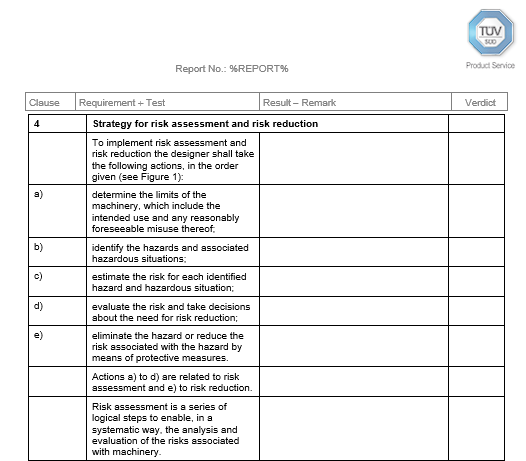
\includegraphics[width=\textwidth]{img/trf.png}

\bigskip \adjustimage{width=\textwidth, center, caption={Test Report Form}, label={fig1}, nofloat=figure, vspace=\bigskipamount}{img/trf.png}

\paragraph{} A more recent approach to risk assessment might be the use of mCom ONE which is being used currently. mCom ONE is a cloud based software solution that facilitates life-cycle management of hazards by bringing machinery, people and processes together while keeping the data readily available for stakeholders across sites \cite{mcom}. mCom ONE provides a centralized platform that allows companies to manage and track their regulatory compliance requirements, including product safety testing and certification, regulatory reporting, and quality control. The platform also provides real-time visibility into compliance status and allows for proactive identification of potential compliance issues. This tool supports engineer in following a checklist based audit to identify hazards according to safety standards. The workflow remains the same instead the TRF is now replaced by its digital counterpart. 

% \bigskip 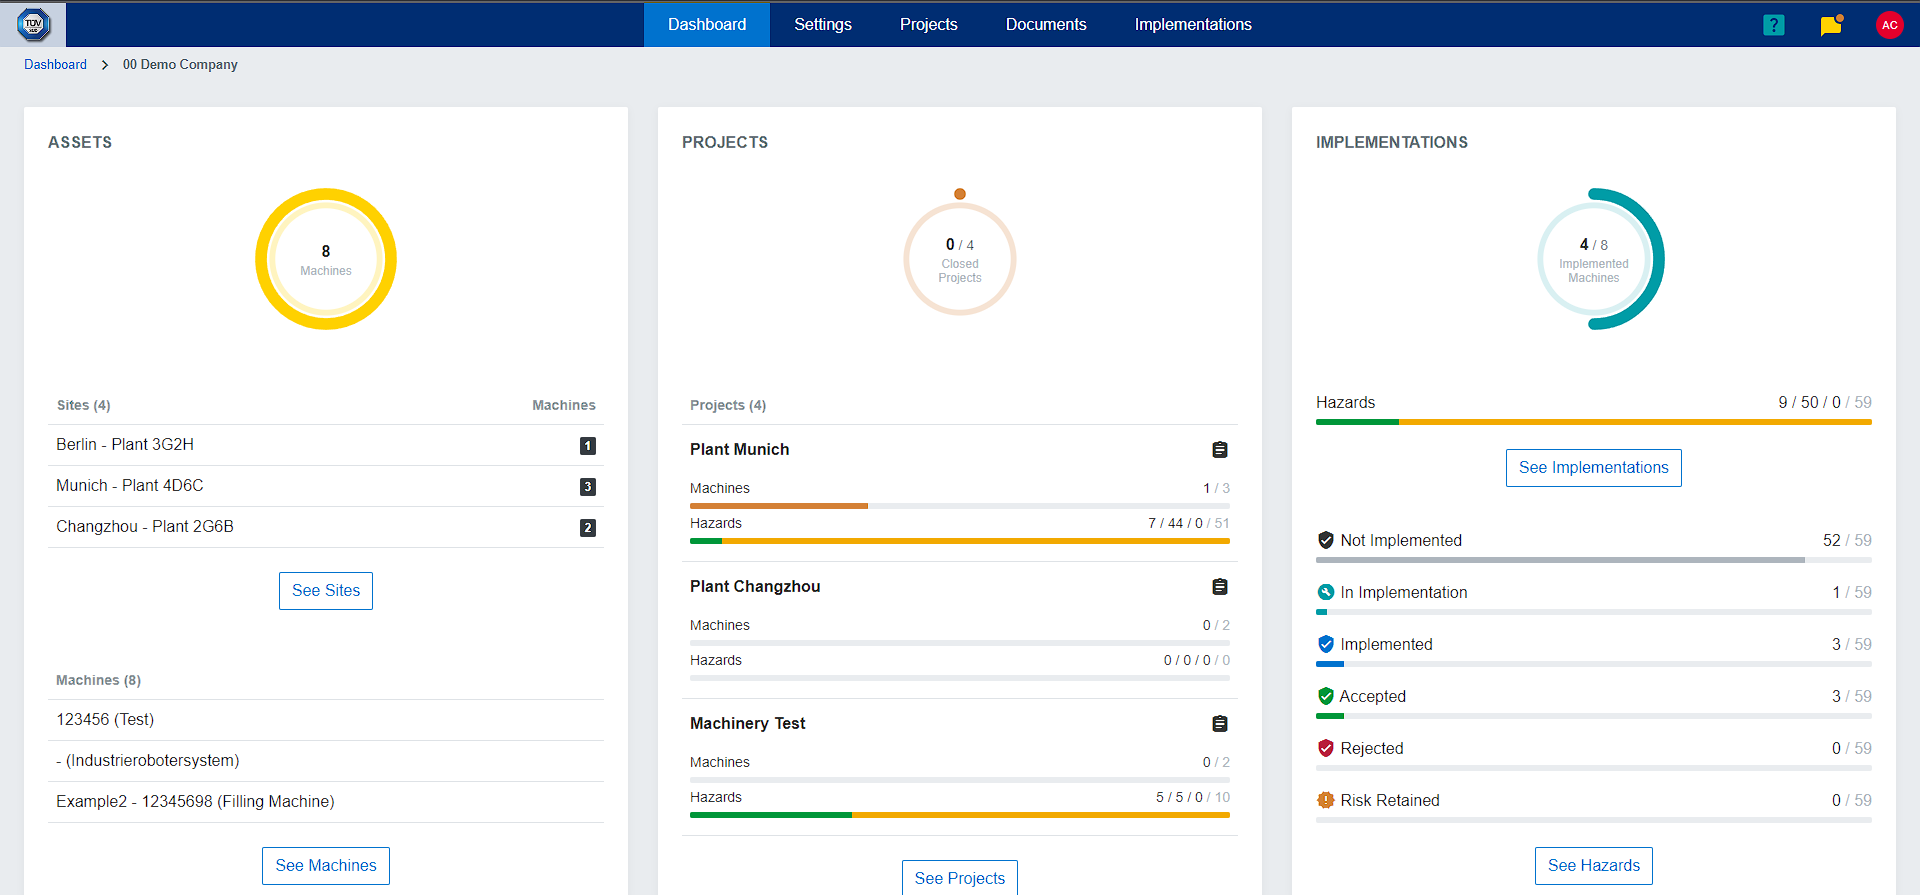
\includegraphics[width=\textwidth]{img/mCom.png}

\bigskip \adjustimage{width=\textwidth, center, caption={mCom ONE dashboard}, label={fig2}, nofloat=figure, vspace=\bigskipamount}{img/mCom.png}

\section{Knowledge model}\label{km}
A knowledge model is a representation of knowledge that captures the concepts and relationships of a specific domain. It is a structured and formal representation of knowledge that can be used to support decision-making, problem-solving, and knowledge management in various applications. As surveyed by Yun et al. \cite{Yun2021}, a knowledge model can be represented in various forms such as semantic networks, ontologies, decision trees, and rule-based systems. It can be used to capture knowledge from experts and documents in a particular field or domain, and then codify and organize that knowledge in a way that can be shared and reused by others.

\paragraph{} A knowledge model can be used in a wide range of applications such as artificial intelligence, knowledge management, and expert systems. In artificial intelligence, knowledge models can be used to represent knowledge in a specific domain to support reasoning and decision-making. In knowledge management, knowledge models can be used to organize and manage knowledge in a particular organization or community. In expert systems, knowledge models can be used to capture the knowledge of experts and automate decision-making processes.

\subsection{How to model knowledge} \label{how_to_model}
According to the studies by Dong et al. \cite{Dong2022} and Yun et al. \cite{Yun2021}, there are many ways to model knowledge, depending on the type and complexity of the knowledge to be represented. Some common approaches to modeling knowledge include:

\begin{itemize}
    \item \textbf{Ontologies:} An ontology is a formal representation of a domain of knowledge that defines the concepts and relationships within that domain. Ontologies are often used to represent complex or specialized knowledge and can be used in applications such as natural language processing and artificial intelligence.
    \item \textbf{Concept maps:}  A concept map is a graphical representation of a domain of knowledge that shows the relationships between different concepts. Concept maps can be used to visualize and organize knowledge, as well as to identify gaps or inconsistencies in the knowledge.
    \item \textbf{Knowledge graphs:}  A knowledge graph is a graph-based representation of structured knowledge that consists of entities (also known as nodes or vertices) and the relationships between them (also known as edges or arcs). Knowledge graphs are often used to represent and organize knowledge in a machine-readable format, and are used in applications such as search engines and recommendation systems.
    \item \textbf{Semantic networks:}  A semantic network is a graphical representation of the meaning of words or concepts in a domain of knowledge. Semantic networks can be used to represent the relationships between different concepts and to understand the meaning of words or phrases in context.
    \item \textbf{Decision trees:}  A decision tree is a graphical representation of a decision-making process that shows the possible outcomes of a series of decisions. Decision trees can be used to model knowledge about decision-making processes and to make predictions or recommendations based on that knowledge.
\end{itemize}

 \subsection{Knowledge modeling in industrial risk assessments} \label{km_in_ira}
 Knowledge models can be used to make industrial risk assessment more efficient by providing a structured representation of the knowledge and information relevant to the risk assessment process. For example, an ontology or a knowledge graph can be used to represent the concepts and relationships related to the industrial processes being studied, the hazards associated with those processes, and the control measures that can be implemented to mitigate those hazards. This structured representation of knowledge can then be used to automate parts of the risk assessment process, such as identifying relevant hazards or control measures, or to support decision-making by providing relevant information at the appropriate stage of the process. Knowledge models can also be used to support the continuous improvement of the risk assessment process by providing a framework for organizing and storing information about past risk assessments, identifying trends and patterns in the data, and tracking the effectiveness of risk control measures over time.
 
 \paragraph{} A knowledge model for industrial risk assessment may include information about the types of hazards associated with different industrial processes, such as mechanical, electrical, vibration, noise, radiation and multiple other hazards. It may also include information about risk reduction measures, preventive measures, testing requirements, that can be used to mitigate these hazards. In addition, a knowledge model for industrial risk assessment may include information about regulations and standards related to industrial safety, such as ISO 12100 and other relevant safety standards. This information can help ensure that risk assessments are conducted in compliance with applicable regulations and standards. 
	\chapter{Related Work} \label{rw}

\bigskip \bigskip To the best knowledge, there exists no prior work which encompasses all research topics together, as addressed in Chapter \ref{rq}. Therefore the related works are discussed topic wise.

\section{Knowledge elicitation}
Acquisition of knowledge and structuring it is itself a form of complex expertise. There are a wide range of techniques and methods that could be used to elicit knowledge from domain experts. The systematic methods to do so are illustrated in the work of Shadbolt et al. \cite{shadbolt2015}. The paper \cite{shadbolt2015} also presents a study on the software tools for knowledge acquisition. The paper focuses on knowledge elicitation in the context of ontology development, from domain experts. 

\paragraph{} Another article by Fenoglio et al. \cite{Fenoglio2022} describes a proposal for tacit knowledge elicitation to capture the best operational practices of experienced domain experts. This paper is based on a mix of algorithmic techniques and cooperation. It provides a functional description of a cognitive framework for capturing knowledge into a knowledge graph.

\paragraph{} The work by N. Jain et al. \cite{text2kg} presents an overall complete work package for automated construction of knowledge graph from raw text. It shows how OpenIE can be used to extract semantic triples directly from text, without the requirement of a formal ontology. This can be beneficial when building a knowledge model from scratch with unstructured text such as documented text as input. Therefore, these works can be referred to work on RQ 2 as given in Chapter \ref{rq}.

\section{Modeling}

The methodologies for the development of knowledge based systems are discussed in the work of Plant et al. \cite{Plant2003}. The "Buchanan's methodology" as cited here is an approach of interest which consists of 5 main phases namely Identification, Conceptualization, Formalization, Implementation and Testing. The problem is first identified, concepts are found to represent knowledge, the concepts are then structured in a formal arrangement, the knowledge is then implemented and tested on use cases to validate the system. The Reformulations, Redesigns and Refinements are based on the Testing phase and accordingly each phase is repeated. 

\paragraph{} There are works which deals with the modeling of knowledge from safety standards. The work presented in \cite{Luo2016} is aimed at model based safety assurance. The novel approach called the "Snowball methodology" described in this PhD thesis provides a rule based technique for developing conceptual model from safety standard. The technique is similar to creating a snowman, starting with very basic concepts that comes from high-level requirements and then just like rolling the snowball in the snow, the size of the model becomes bigger with more concepts and relations adding up to the model.

\paragraph{} In the work presented in \cite{Bunte2020}, an interoperability of semantic models in modular production systems is given. An ontology based approach is used to create a semantic model for individual modules, combined into an overall model. The data can be transferred to individual modules through the semantic model, which would play as an interface. This improves adaptability without manual effort. The use case, as presented in this PhD work, would be beneficial for faster re-assessments of product in safety and security assessments. If this similar use case is considered for the communication of information related to performance level from the semantic model to the actual machine, an M2M communication is achieved. This can be a two step approach, first find the missing information regarding performance level and then an automatic communication to the connected machines. Then if risk persists it can be mitigated automatically if possible, otherwise an alarm might be set. This can be an ultimate goal to reach towards automated risk assessment and can be a topic of future research. However, for this thesis, only finding the missing information related to performance level is focused on and the M2M communication is left for future work. Hence, \cite{Bunte2020} is useful for RQ 3 given in Chapter \ref{rq}.

\section{Validation}

According to Luo \cite{Luo2016}, validation by domain expert is a necessary final step of model development. A formal representation of the conceptual model is an excellent
basis for validation. Generating checklist from the given knowledge graph is a desirable achievement for faster risk assessment. This can also serve the purpose of validation. Paper \cite{9297991} introduces an ontology based approach for automating the generation of questions from an RDF graph. Information from the ontology is broken down into categories in the format of SPARQL queries. The queries are then converted into questions by the algorithm described in the paper.

\paragraph{} The work of R. Roy et al. \cite{Roy2004} also involves domain experts in the process of model validation. The work also presented a validation questionnaire for the experts to record their impression of the model and present a quantitative outlook of the model.
	\chapter{Methodology} \label{method}

\bigskip \bigskip A systematic approach towards development of a knowledge model can be found in the works of Roy et al. \cite{Roy2004} and Plant et al. \cite{Plant2003}. However, for the purpose of this thesis, developing a knowledge model for industrial risk assessments involves a systematic approach that includes the following steps:
\begin{itemize}
    \item \textbf{Scope and purpose of the knowledge model:} The first step is to identify the specific processes, products, and systems that will be covered by the knowledge model. The purpose of the knowledge model should also be clearly defined, including the type of risk assessment it will support and the stakeholders who will use it. This section of the thesis mainly deals with RQ 1 and evaluates Hypothesis 1.1.
    \item \textbf{Gather relevant data:} The next step is to gather relevant data from various sources. Knowledge from safety standards and knowledge from experts are the main source of knowledge for this work. The data should be organized in a structured format that can be easily searched and analyzed. 
    \item \textbf{Define the knowledge model:} The knowledge model should be designed to capture the relevant information from safety standards, products covered and knowledge from experts. This includes defining the entities, attributes, and relationships that are important for risk assessment.
    \item \textbf{Develop the knowledge model:} Once the knowledge model has been defined, it can be developed using a variety of methods and tools to support the chosen method. Different methods to model knowledge are defined in Section \ref{how_to_model}. This part mainly deals with RQ 2 and evaluates Hypothesis 2. 
    \item \textbf{Implement the knowledge model:} The knowledge model should be integrated into the current risk assessment process. By doing this it becomes easier to validate the model and its output. This involves working for RQ 3 and evaluate Hypothesis 3.1.
    \item \textbf{Validate the knowledge model:} The knowledge model should be validated to ensure its accuracy and reliability. This section of the thesis mainly deals with RQ 4 and evaluates Hypothesis 4.
    \item \textbf{Maintain and update the knowledge model:} It should be possible to regularly review and update the knowledge model to ensure that it remains current and relevant. This may involve incorporating new data or knowledge, refining the model based on feedback from users, or updating it to reflect changes in safety standards or regulations. Also for future applications it should be easy to grow the model with newer safety standards and risk assessments.
\end{itemize}

The implementation and validation of the knowledge model are not really a part of the methodology to build the knowledge model. These topics would come after the model is built, so they are considered as separate chapters after methodology. Also, maintenance and updating the knowledge model is discussed in between other topics. So, it is not separately discussed.

\paragraph{} Developing a knowledge model for industrial risk assessments requires a multidisciplinary approach that involves dealing with data from risk assessments, semantic data from safety standard and exploring the field of Natural Language Processing to reduce manual effort in the process. Also developing the knowledge graph from scratch involves the idea of ontology and semantic triples which are explained further in this chapter.

\section{Scope and purpose of the knowledge model} \label{scope}

\subsection{Scope of the model}
For this project, Hypothesis 1.1 proposed can be considered effective and Hypothesis 1.2 can be nullified as it is a customer-centric approach. Hypothesis 1.2 considers developing the knowledge model from engineering files of each customer which is specific to machine type. This approach may focus too heavily on meeting the customer's needs and expectations, for the particular machine used potentially overlooking important safety considerations. This can lead to a higher risk of accidents that could have been prevented. Also this approach rejects the idea of reusing previous risk assessments which does not make it a fast and efficient approach for future risk assessments. On the other hand, Hypothesis 1.1 is a project-centric approach and can be applicable for machinery of multiple customers. This approach is based on safety standards which are generalized. The following arguments can be made in favour of Hypothesis 1.1:
\begin{enumerate}
    \item Safety standards are based on industry-wide best practices and regulatory requirements, which means they are developed by experts and have been proven effective in promoting safety and reducing risk. 
    \item A safety standard-centric approach is more comprehensive and covers a wider range of potential risks and hazards. It takes into account not only the customer's needs and expectations, but also the broader context in which the product or service is being used.
    \item Safety standards are legally binding, which means that organizations are required to comply with them. By using a safety standard-centric approach, organizations can ensure that they are meeting their legal obligations and reducing the risk of liability.
    \item Safety standards are regularly reviewed and updated, which means that a safety standard-centric approach can help organizations stay up-to-date with the latest best practices, new hazards and requirements. This is in contrast to the engineering files approach of Hypothesis 1.2, as these data stays constant for the given machine, even if new hazards for the machine type are found later.
    \item Expert knowledge can bring a broader perspective to risk assessment, incorporating information from previous assessments can make the future assessments faster. The expert's interpretation of the standard can help to identify potential hazards and develop more effective mitigation strategies which can be transferred to the knowledge model to make it more effective to use.
\end{enumerate}

So, the knowledge model for faster and efficient industrial risk assessment can be made by digitizing knowledge from domain experts and safety standards. This establishes the ground on which the knowledge model is built.

\subsection{Purpose of the model}
The risk assessment of a laser cutting machine is considered for this thesis. A Type A standard, the EN ISO 12100:2010 is used. A documentation of a previous assessment on the machine in accordance with EN ISO 12100:2010 is used as an expert's knowledge, that can be elicited for developing the knowledge model.

\paragraph{} The purpose of a knowledge model built using knowledge from domain experts and safety standards would be to improve safety and reduce risk. Also to make industrial risk assessments faster and efficient. The model would incorporate relevant safety standards and guidelines, as well as the results of previous risk assessments and expert's interpretation, to provide a comprehensive understanding of potential hazards, preventive measures, location of hazards, risk measure, reason of occurrence, mitigation strategies and other important information that is segregated for each hazard. Now this becomes easier for the engineer to look for the hazard applicable for the machine, search for the preventive measures from the knowledge model and mitigate them easily. This approach is faster and efficient than going through the huge safety standard documents and then interpreting the standard to assess the machine. The model should also be future-ready for applications like machine-to-machine communication as discussed further later in this thesis \ref{m2m}.

\section{Gather relevant data}
\label{gather_relevant_data}

There are two main source of data which are considered for the knowledge model,
\begin{itemize}
    \item Knowledge from safety standard
    \item Knowledge from expert
\end{itemize}

\subsection{Knowledge from safety standard}
Safety standards are usually lengthy and complex documents, and extracting knowledge manually can be a tedious task. However, there are several techniques available in computer science that can be used to automate the process of extracting knowledge from safety standards. Here are some of the techniques that can be used:
\begin{itemize}
    \item \textbf{Natural Language Processing (NLP):} NLP is a technique used to extract information from natural language texts such as safety standards. NLP algorithms can be used to automatically identify the key concepts and relations between concepts, from the safety standards. The concepts and relations can then be used to create structured data that can be easily analyzed.
    \item \textbf{Machine Learning (ML):} ML algorithms can be trained on safety standards to identify patterns and extract information automatically. For example, ML algorithms can be used to identify safety hazards and controls, and categorize them according to their severity.
    \item \textbf{Data Mining:} Data mining techniques can be used to extract information from large datasets of safety standards. These techniques can help identify patterns and relationships in the data, which can be used to develop a comprehensive knowledge model.
\end{itemize}

The machine learning approach and data mining approach are data-intensive. It means that these two techniques need a huge quantity of data to train and test the model. These approaches are useful when there is a large amount of structured data available, such as safety concepts and the relations between the concepts. However, in this project, the only available data source is the EN ISO 12100 safety standard which contains unstructured textual data that is not machine readable. The idea here is to develop such a structured data source that can be used in future by machine learning applications.

\paragraph{} On the other hand, natural language processing (NLP) techniques can be useful when there is limited data available, which is unstructured. NLP techniques can help to identify key concepts and relations from safety standard based on the language used in the document. However, it's important to note that each approach has its own strengths and limitations. For example, ML and data mining approaches may be able to identify complex patterns and relationships in the data that are not easily recognizable through NLP techniques. Similarly, NLP techniques may not be able to identify and connect all safety hazards and controls, concepts and relations that are present in the safety standard.

\paragraph{} Therefore, the best way to go is semi-automatic, which is followed in this work. An NLP algorithm can be helpful to automate the process of information extraction from safety standards, but the process is still heavily dependent on manual effort. This is because safety standards are often complex documents that may contain nuanced information that may be difficult for the NLP algorithm to fully capture. Manual work can help ensure that the extracted information is accurate and relevant to the specific context. This can include reviewing and refining the results of NLP techniques to ensure that they accurately reflect the content of the safety standards. A combination of NLP technique and manual work may be the best approach for developing a comprehensive knowledge model for safety standards and this can help ensure that the extracted information is accurate, relevant, and tailored to the specific context.

\subsubsection{Information extraction pipeline}
An information extraction (IE) pipeline is a series of steps or processes designed to extract structured information from unstructured data, such as text documents. From the work of N. Jain et al. \cite{text2kg} and from the projects demonstrated in \cite{analyticsvidhya} and \cite{medium}, the following pipeline is prepared.

% \bigskip 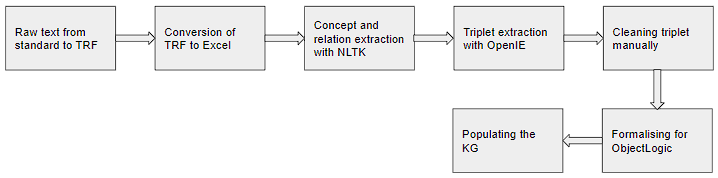
\includegraphics[width=\textwidth]{img/12100_IE_pipeline.png}

\bigskip \adjustimage{width=\textwidth, center, caption={IE pipeline for the safety standard}, label={fig3}, nofloat=figure, vspace=\bigskipamount}{img/12100_IE_pipeline.png}

\paragraph{} The first step is to extract the text from the safety standard which is in .pdf format to a more workable .xlsx format. This is done using a tool which is used to convert a pdf document into a TRF (Test Report Form) and then from the TRF to an excel sheet using a simple Python code. This de-tour for the conversion of the standard from .pdf to .xlsx is used so that the formatting of the original document is preserved. This ensures that the information under each clause as described in the standard is also preserved in the .xlsx format. It ensures that the triplets are created under each clause separately and thus makes the cleaning easier. The TRF or Test Report Form is the document used by experts to perform safety assessment on a machine according to a standard. The excel sheet prepared have the clause numbers on separate column and the requirements on another column. Each requirement per clause is separated by each row. This makes working with the text much easier for the subsequent steps. The effort required is also minimum since the process is automated. 

\paragraph{} Now that the requirements from the standard are extracted in a separate column and each requirement separated into rows, few data cleaning steps must be taken to ensure that the NLP algorithm returns workable results. The information that are not required such as Notes, Examples, Tables, Figures and other data that need not be a part of the final knowledge model can be excluded. This curated column can finally be converted to a pandas dataframe to be an input of the NLP tool used. While researching for this work, there are several tools and libraries found that can assist with various steps in the process of generating a knowledge model from unstructured text, these are:
\begin{itemize}
    \item \textbf{NLTK:} This is a popular Python library for natural language processing, which includes tools for text preprocessing, named entity recognition (NER), and part-of-speech (POS) tagging.
    \item \textbf{Stanford CoreNLP/Stanza:} This is a Java library for NLP that includes tools for tokenization, part-of-speech tagging, dependency parsing, and named entity recognition. A newer version of this package is Stanza which is a Python package and CoreNLP can also be accessed by Stanza via its server interface by launching the Stanford CoreNLP client. 
    \item \textbf{Spacy:} This is another popular Python library for NLP that includes tools for text preprocessing, named entity recognition, part-of-speech tagging, and dependency parsing.
    \item \textbf{OpenIE:} This is a tool for extracting open-domain, subject-predicate-object (SPO) relation triples style information from text, which can be used to construct a knowledge graph. This tool is originally from the Stanford CoreNLP package which can also be accessed via Stanza in a Python environment.
    \item \textbf{ClauseIE:} Clause-based Information Extraction is a type of information extraction technique that focuses on extracting information from specific clauses in text. This tool is the work of Corro et al. \cite{Corro2013}.
\end{itemize}

\subsubsection{Concepts and relation extraction using NLTK}
NLTK (Natural Language Toolkit) provides a variety of tools and methods for extracting concepts and relations from sentences. One approach to extracting concepts and relations from sentences using NLTK involves part-of-speech (POS) tagging. POS tagging is the process of assigning a part-of-speech tag (such as noun, verb, adjective, etc.) to each word in a text document. The goal of POS tagging is to identify the grammatical structure of the text and to disambiguate the meanings of words based on their context. NLTK provides built-in functions for performing POS tagging on texts. Using NLTK, first POS tagging is performed on each sentence to identify the parts of speech of the words in the sentence. Then, rules or patterns are applied to the POS tagged sentence to identify concepts and relations. Here, nouns of all kinds are put to a list as concepts and verbs of all kinds are put to a list as relations. \cite{nltkbook}

\subsubsection{Triple Extraction with OpenIE}
OpenIE (Open Information Extraction) is a technique in natural language processing (NLP) that is used to extract structured information from unstructured or semi-structured text. Unlike traditional named entity recognition (NER) or relation extraction techniques, OpenIE aims to extract relations between entities in a more open-ended and unconstrained way, without relying on pre-defined relation types or hand-labeled training data. OpenIE is often used as a preprocessing step for building knowledge graphs, since it can help automatically identify relationships between entities in large amounts of unstructured text which is demonstrated by the work done by N. Jain et al. \cite{text2kg}. Similar use of OpenIE is done in this work with Stanford CoreNLP OpenIE.

\paragraph{} SPO (Subject-Predicate-Object) triples are a way of representing structured information in a way that can be easily understood and processed by computers. Each SPO triple consists of three components:
\begin{itemize}
    \item \textbf{Subject:} The entity or concept being described
    \item \textbf{Predicate:} The relationship or property between the subject and the object
    \item \textbf{Object:} The entity or value that the subject is related to by the predicate
\end{itemize}
SPO triples are useful for building knowledge models because they provide a way to represent structured information in a machine-readable format. By representing information in terms of SPO triples, a knowledge graph can be built that allows us to make inferences, answer questions, and discover new insights based on the relationships between entities. 

\paragraph{} Since Python is used for this project and Stanford CoreNLP provides OpenIE in the Java environment, a newer Python package from Stanford NLP called Stanza is used. Stanza allows accessing the Java toolkit via its server interface. First the filtered sentences from the dedicated column of the excel sheet is taken as an input and converted to a pandas dataframe to make work easy. Then CoreNLP Server is launched in the background with the annotator as OpenIE sending each sentence from the dataframe to the server one by one. The output for each line is then appended to a dictionary tagging each subject, relation and object separately. For each line there may be more than one triple so the triple dictionaries are appended to a triples list which is the final output for each sentence. This particular structured format of using dictionaries is used so that the process of formalization of the triples to build the final knowledge model could become automatic and simple, which is discussed later in this chapter. Finally each list for each line is written automatically in the working excel. Here, excel is used because of its familiarity and ease of use. The final aim is to prepare the data set to be fed into OntoBroker which is used to prepare the semantic model. Working code for the CoreNLP Client Interface can be cited from the work of P. Qi et al. \cite{stanza}. An example from the safety standard might make the complete process clearer. 
\begin{itemize}
\item Sentence: "Risk analysis provides information required for the risk evaluation, which in turn allows judgments to be made about whether or not risk reduction is required."
\item 'subject': 'Risk analysis', 'relation': 'provides information required for', 'object': 'risk evaluation'
\item 'subject': 'Risk evaluation', 'relation': 'allows judgements to be made', 'object': 'risk reduction'
\end{itemize}

\subsubsection{Manual work}
It is found that the triples generated using OpenIE had a wide variation of SPO combinations for a single sentence. For some sentences the triples generated can be used for building the knowledge model but for some sentences the triples made no sense. Also for some sentences there was no output. The more complex a sentence gets, the more difficult it becomes for the algorithm to give a correct output. This leaves a sweet spot for future research on this topic about how an algorithm can be optimized for automatic generation of SPO triples from unstructured text. However, for the course of this work, manual intervention is required to get the final triples right.

\paragraph{} For sentences where the SPO triples were not extracted correctly, a manual extraction of triples is required. Extracting SPO triples manually from this standard involves reading through the individual sentences and understanding its linkage with neighbouring sentences. Here are some general steps followed:
\begin{itemize}
    \item Read the safety standard: The document is read carefully to understand the context and structure of the content. Most importantly to understand how the clauses are divided and their content.
    \item Identify the relevant information: The information is identified that is relevant to the risk assessment process, such as hazards, risks, preventive measures, and other safety requirements.
    \item Identify the subject: The subject or entity is identified that the information is referring to. This could be a machine, hazard name, process, or other element related to the machinery design.
    \item Identify the predicate: The predicate or relationship between the subject and object is identified. This could be a requirement, recommendation, or other type of relationship.
    \item Identify the object: The object or attribute related to the subject is identified. This could be information on hazard, risk reduction measure, safety requirement information, or other relevant information.
    \item Organize the information into SPO triplets: Once the subject, predicate, and object are identified, the information is organized into SPO triplets in the dictionary format as discussed previously.
\end{itemize}

Here's an example of an SPO triplet that couldn't be extracted automatically, but needs to be extracted manually from the ISO 12100:
\begin{itemize}
    \item Sentence: Electrical hazards - For requirements related to specific machines, see corresponding IEC standards (for example, IEC 61029, IEC 60745 or IEC 60335).
    \item Subject: electrical hazards
    \item Predicate: reference standards
    \item Object: IEC 61029, IEC 60745, IEC 60335
\end{itemize}
    
This information can be organized into an SPO triplet as follows:

[{'subject': 'electrical hazards', 'relation': 'reference standards', 'object': 'IEC 61029'}]

[{'subject': 'electrical hazards', 'relation': 'reference standards', 'object': 'IEC 60745'}]

[{'subject': 'electrical hazards', 'relation': 'reference standards', 'object': 'IEC 60335'}]

\subsection{Knowledge from expert}

% \bigskip 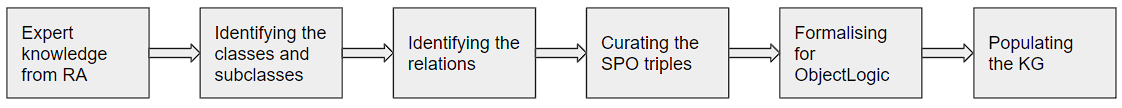
\includegraphics[width=\textwidth]{img/Expert_IE_pipeline.png}

\bigskip \adjustimage{width=\textwidth, center, caption={IE pipeline for the knowledge from expert}, label={fig4}, nofloat=figure, vspace=\bigskipamount}{img/Expert_IE_pipeline.png}

\paragraph{} For this thesis, the risk assessment of a laser cutting machine is considered. The work of Kleen \cite{kleen} is taken as a documentation of previous risk assessment that is done on the laser cutting machine concerned. This machine consists of individual components like robot, laser, transfer station on which risk assessment in accordance with the EN ISO 12100 was performed. These individual reports can be considered to be the knowledge from an expert that is required to build the model. Expert knowledge elicitation from documents involves a process of extracting, categorizing, and organizing information to generate insights and knowledge that can be used to develop the knowledge model. Mostly, the information is in tabular format so unlike the plain textual data from the safety standard, this data is somewhat semi-structured. It is required to understand the structure and identify the pattern that could be used to amalgamate the knowledge from two sources so that the knowledge model could have a homogeneous structure. For example, relations (predicates) are looked for which can match the ones extracted from the safety standard. This matching is done manually to avoid similar meaning triples to be represented differently in the final knowledge model. The data is organized similarly as done for the safety standard, that is, by creating SPO (Subject-Predicate-Object) triples in a dictionary structure. 

\section{Define the knowledge model}\label{class_hierarchy}

After extracting the required data in a structured format, it is required to define a basic outlined structure of the knowledge model. A class hierarchy diagram can be helpful here. A class hierarchy diagram is a visual representation of the classes and their relationships in an object-oriented system. Classes and sub-classes can provide a hierarchical structure and organization to the data represented by the SPO triples. The class hierarchy diagram can help to visualize the concepts of the knowledge model and most importantly which concept is derived as a subclass from which parent concept. Additionally, a class hierarchy provides a way to define and enforce consistency within the knowledge model. By defining a set of classes and sub-classes, a common vocabulary and structure can be established that can be used throughout the knowledge model. This can help to ensure that the knowledge model is consistent and easy to understand. 
% Not all relations between the concepts show a "is a" relation so it can be called to be "partly an ontology".

\paragraph{} Inspiration from the work of Luo \cite{Luo2016} is taken to prepare the outline of the model. The "Snowball approach" as Luo mentioned in his work, the high level concepts are the ones to begin with. Then just like rolling a snowball, as the model grows, the concepts get much more targeted to low level concepts with the possibility to grow each child node further more. The complete class hierarchy diagram is given on the next page.

% 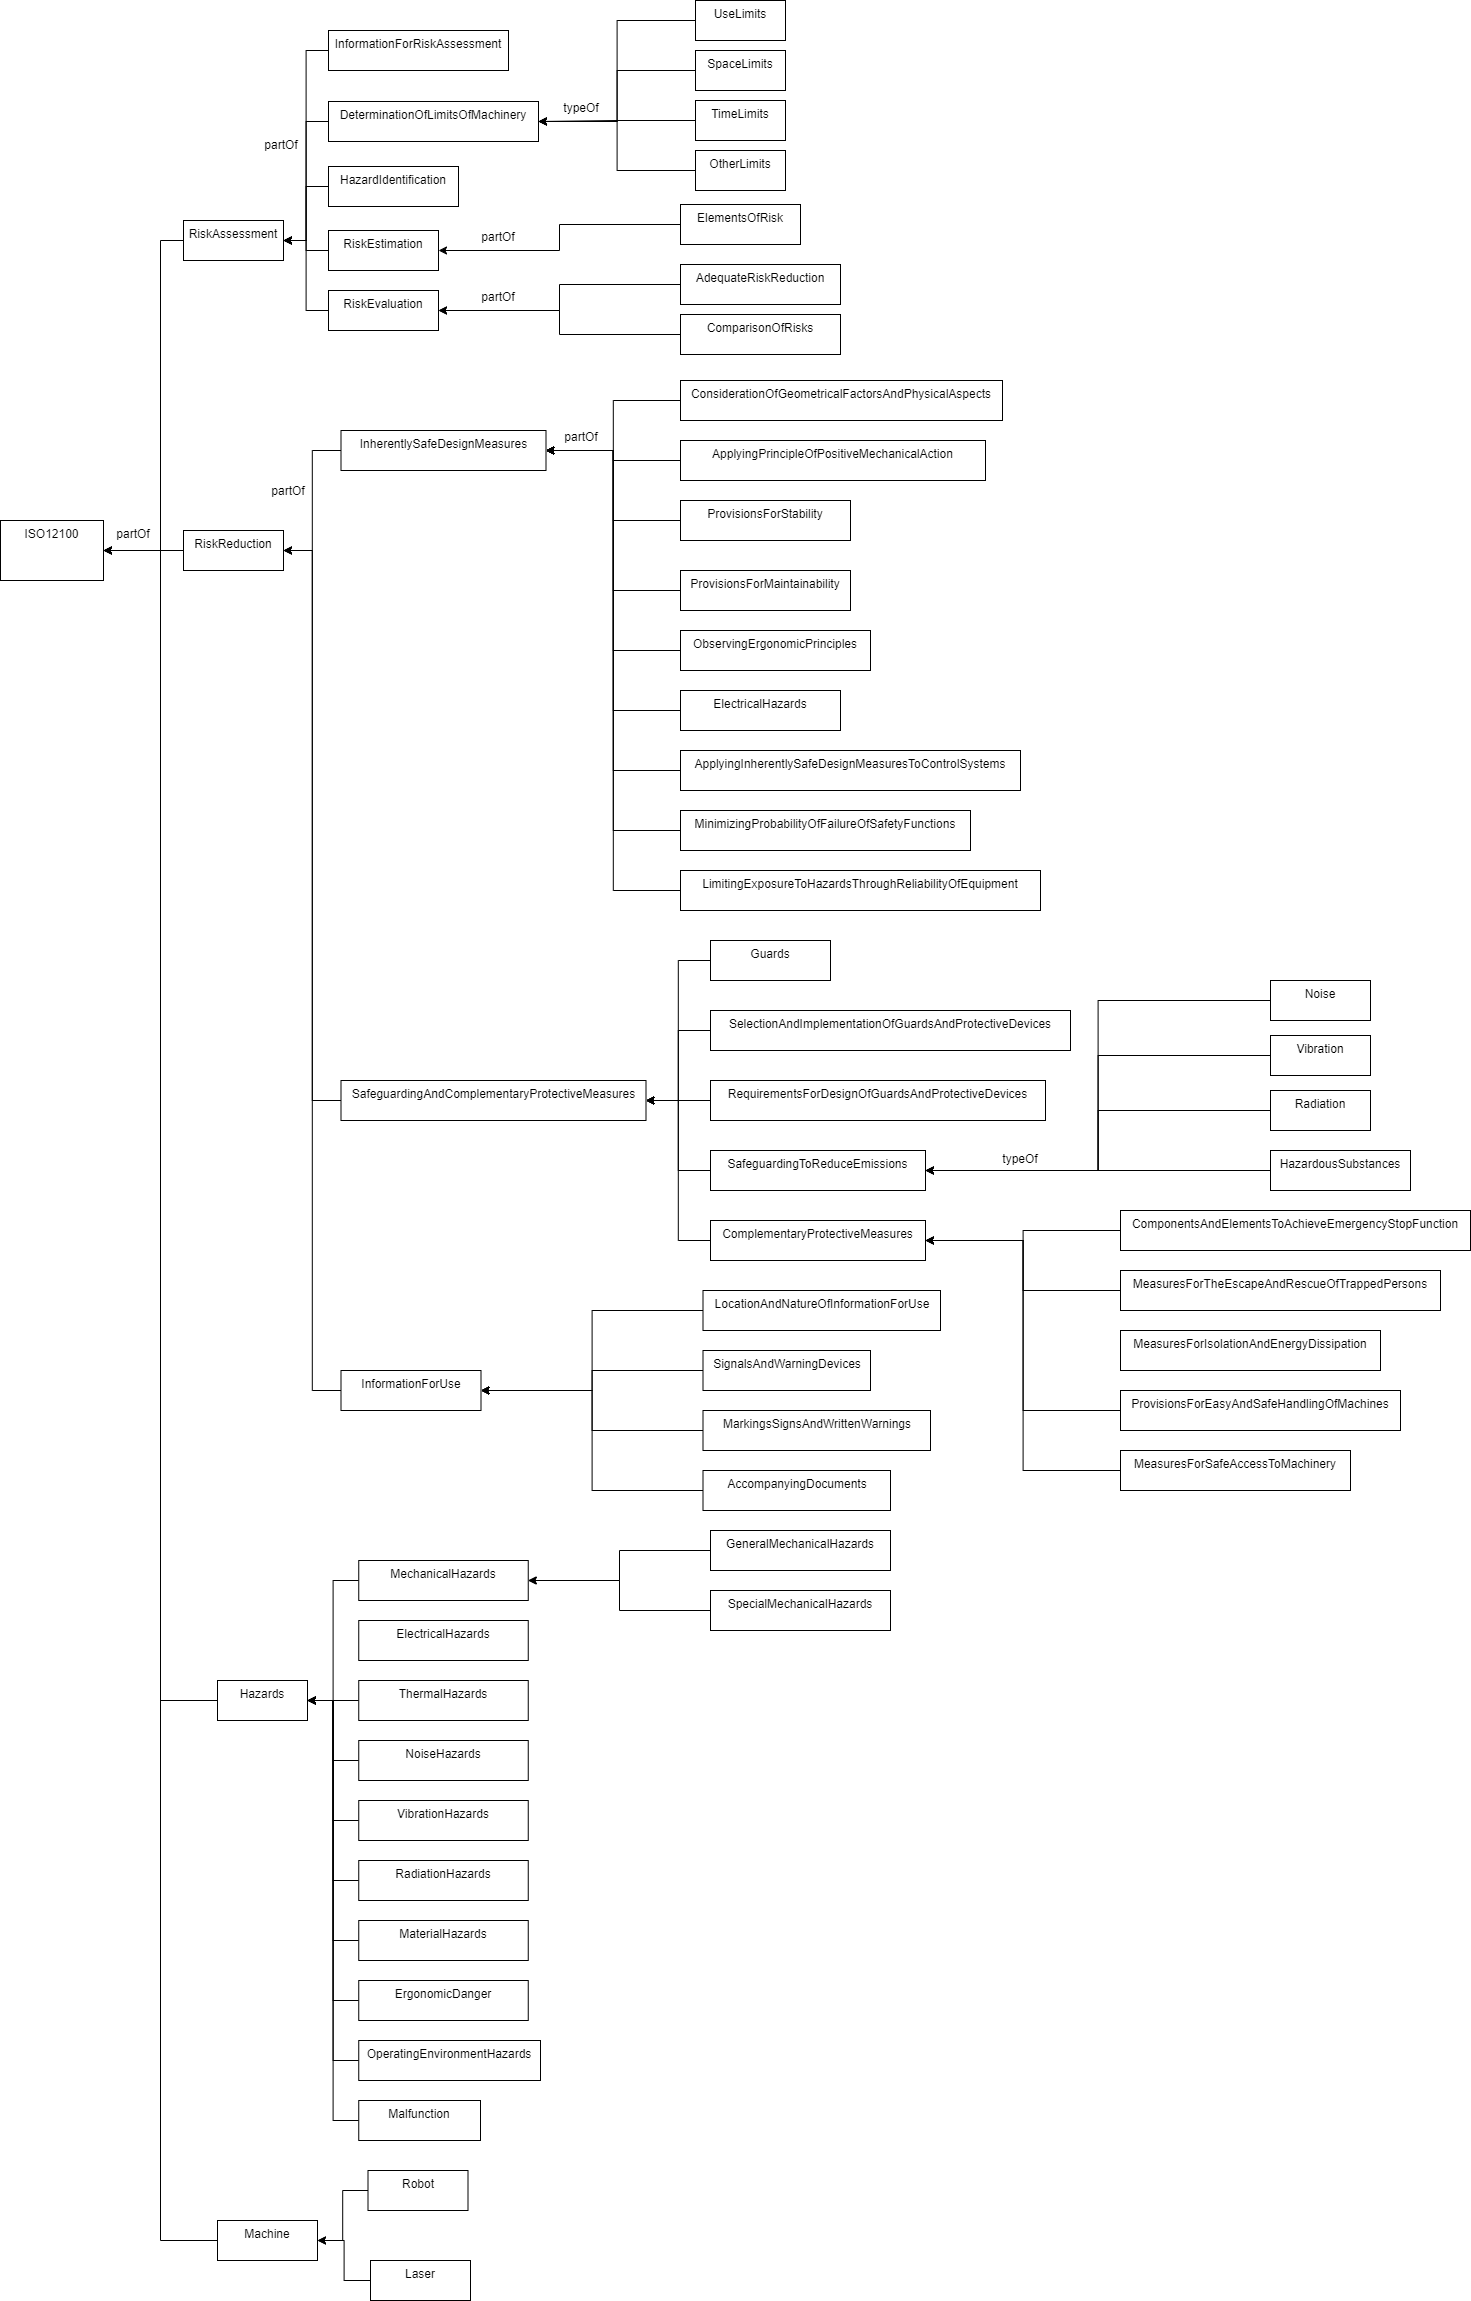
\includegraphics[width=\textwidth]{img/Class_Hierarchy.png}

\paragraph{} For this thesis, the model defined starts with a broad concept "ISO12100". However, it is possible to go on higher level than this if more safety standards are to be added to the model. For example, with the concept "Safety\_Standards" as a level before and child concepts like "Type\_A\_Standards", "Type\_B\_Standards", "Type\_C\_Standards" and then under "Type\_A\_Standards" would come "ISO12100". This could be useful if a knowledge model for other safety standards are also created for different types of standards.

%\bigskip
%\begin{center}
%   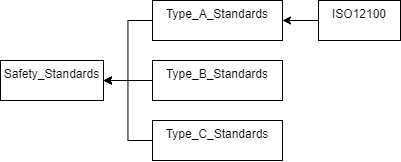
\includegraphics[scale=0.5]{img/Model_Extent.png}
%    %\caption{Possibility of extension on a higher level}
%\end{center}

\bigskip \adjustimage{scale=0.5, center, caption={Possibility of extension on a higher level}, label={fig5}, nofloat=figure, vspace=\bigskipamount}{img/Model_Extent.png}

\paragraph{} To understand the depth of the model, one Instance could be taken as an example. ISO12100 has a sub-class RiskReduction which has a sub-class SafeguardingAndComplimentaryProtectiveMeasures which has a subclass ComplimentaryProtectiveMeasures and finally MeasuresForSafeAccessToMachinery.

% \bigskip\bigskip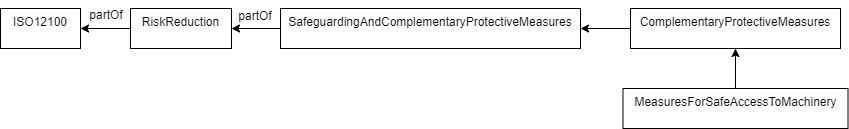
\includegraphics[width=\textwidth]{img/Model_Depth.png}
    %\caption{Depth of the class hierarchy}

\bigskip\bigskip \adjustimage{width=\textwidth, center, caption={Depth of the class hierarchy}, label={fig6}, nofloat=figure, vspace=\bigskipamount}{img/Model_Depth.png}

\adjustimage{width=\textwidth, center, caption={Class hierarchy diagram}, label={fig7}, nofloat=figure, vspace=\bigskipamount}{img/Class_Hierarchy.png}
    
\section{Develop the knowledge model}\label{develop}

Now since the basic outline is drafted, it is required to formalize the information into a knowledge model. OntoBroker \cite{ontobroker} from Semafora Systems is the tool that is used to formalize the SPO triples into a knowledge graph. 

\subsection{Semantic tools used}

\paragraph{OntoBroker: } OntoBroker is the semantic middleware that is used for this project. OntoBroker is a software tool developed by Semafora Systems, which is used for managing and querying ontologies. An ontology is a formal representation of the knowledge in a particular domain, which includes concepts and their relationships, properties and axioms that define these concepts. OntoBroker provides a comprehensive framework for ontology management that includes ontology editing, browsing, querying, and reasoning capabilities. OntoBroker supports multiple ontology languages including OWL, RDF, ObjectLogic. 

\paragraph{ObjectLogic: } ObjectLogic is the primary language for OntoBroker and it is also the language used for this project. ObjectLogic \cite{obl} is a knowledge representation and query language. It explicitly supports data types and have a clean syntax which is easy to understand. In ObjectLogic, knowledge is represented using objects, which have attributes. Objects have relationships to other objects. These objects can be used to model concepts. For the domain of industrial risk assessment, hazards, preventive measures, risks, cause of hazards, etc. are all concepts. ObjectLogic also includes features for defining and reasoning with complex class hierarchies. The complete class sub-class hierarchy is modelled as defined previously in \ref{class_hierarchy}. The main reason of using ObjectLogic is due to its simple syntax which is easy to use even by someone who is not well versed with coding. This makes it easier for the engineers to also contribute and update the knowledge model very easily.

\paragraph{OntoStudio-X: } The development environment used for this project is OntoStudio-X (OSX) \cite{osx}. OntoStudio-X stitches together the advantages of two well-established technical worlds - the tabular format of Microsoft Excel and the inference engine OntoBroker. Through the integration of OntoBroker's function and data structures with Excel's internal object model, it is possible to access all of OntoBroker's functions within the Excel cell structure without the need for Excel VBA. As a result, Excel files containing OntoBroker ontologies and instruction structures can be shared without macros, just like any other .xlsx file. 

% Give screenshots of OSX 3 tabs, 

\subsection{Development of the knowledge graph}

% cite some paper

A knowledge graph is a database that stores and organizes information about concepts or entities (such as people, places, or things) and the relationships between them. Unlike traditional databases that store data in tables, knowledge graphs represent data as nodes and edges in a graph structure. Each node represents an entity and each edge represents a relationship between two entities. General information about a knowledge graph can be cited from the work of Hogan et al. \cite{Hogan_2021}. For example, a knowledge graph might represent a machine as a node and the hazard linked to it as an edge connecting it to another node representing the hazard name which can further be expanded to have information about the preventive measures against the hazard, location of the hazard and so on that can actually help in speeding up the risk assessment process. This makes a knowledge graph to be a perfect candidate to be used for this project. Also the data collected is in SPO format makes the work much simpler to achieve a knowledge graph pertaining to their similar structure. Hence, Hypothesis 2 proposed can be considered to be effective.

\paragraph{} Until this point, the unstructured data from the safety standard and expert's documented knowledge is already collected in a structured format as SPO (Subject-Predicate-Object) triples. Now it is required to formalize this data according to ObjectLogic's syntax to develop the final knowledge graph. An automatic approach is preferred to do so using a Python script. It is beneficial to follow this approach for the following reasons:
\begin{enumerate}
    \item \textbf{Consistency: }A Python script can be used to formalize SPO triples into a knowledge graph with a consistent structure, ensuring that all the data is organized and stored in a standardized manner. This makes it easier to analyze and extract insights when querying the data. For this project, the camel case naming convention is used in general. The upper camel case is considered for the concepts (- subjects and objects) and the lower camel case for the relations.
    % Example flowchart visual
    \item \textbf{Automation: }Using a Python script to formalize SPO triples into a knowledge graph can automate the process, which saves time and reduces the risk of errors that can occur when manually entering data into a graph.
    \item \textbf{Flexibility: }Python is a versatile language that offers a wide range of tools and libraries for data processing and analysis. This makes it easily possible to customize the script to suit specific requirements, such as filtering or transforming the data before or even after it is added to the knowledge graph. Even while building the knowledge model at times it was required to change the format of few data. These changes were done very easily by the code that is used to transform the SPO triples to knowledge graph.
    \item \textbf{Scalability: }Formalizing SPO triples into a knowledge graph using a Python script can be scaled up to handle large volumes of data. This makes it really easy for future expansion of the knowledge graph with several other safety standards.
\end{enumerate}

The column containing the SPO triples from the excel sheet is taken as input. The triples are already structured in a dictionary with the subject object and relation tagged separately. The list of dictionary is looped through to work on each content of the list. First the naming convention is taken care of. Each phrase is split for words and then the first letter of each word is capitalized. Then all the letters are joined together into a single string. For the function of upper camel case, which is used for the subjects and objects, all the initial letters of each word are capitalized and for the function of lower camel case, which is used for the relations, all the initial letters of each word are capitalized except the first word. After naming, the concepts and relations are structured into the schema defination of ObjectLogic as defined in \cite{obl}. The list of formatted output is taken into a pandas dataframe so that it is easier to write on the Excel interface of the OntoStudio-X. A screenshot of the schema in OntoStudio-X is shown below:

% \bigskip\bigskip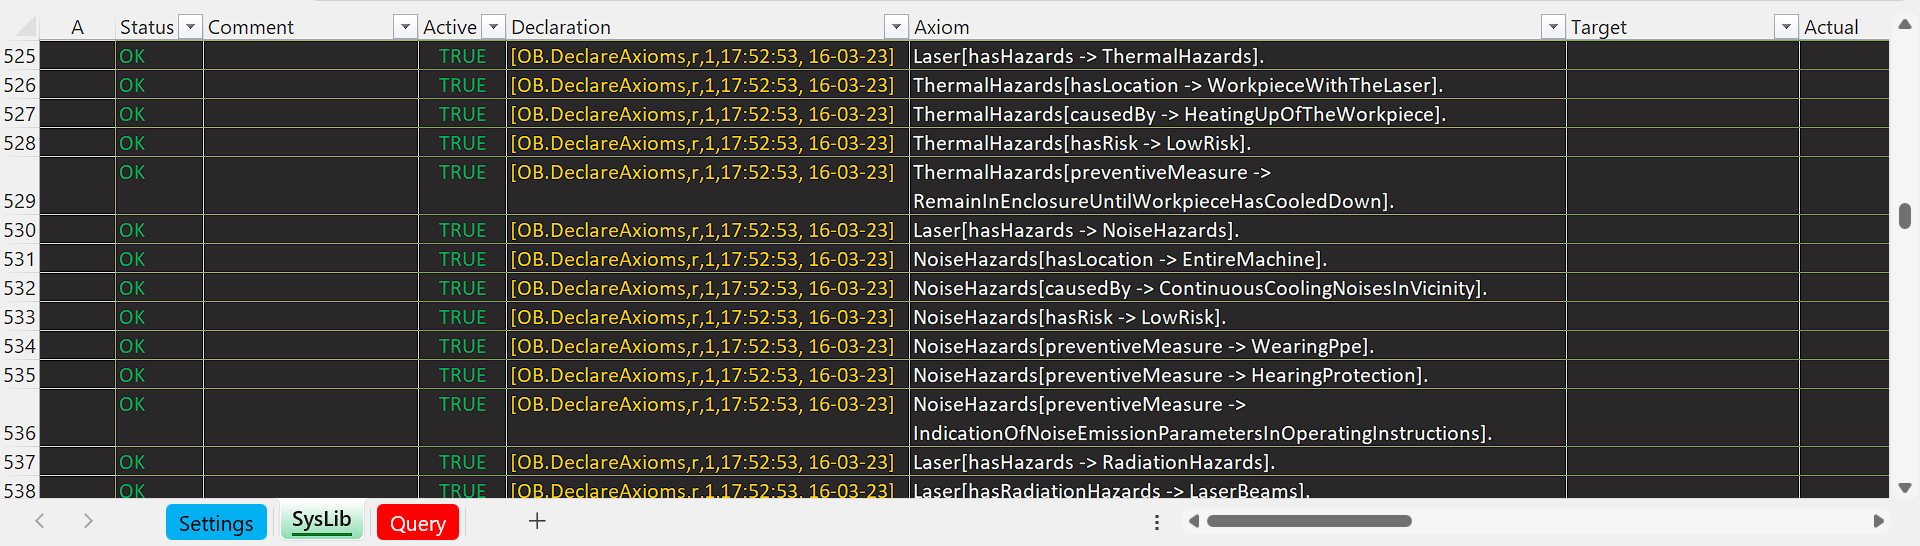
\includegraphics[width=\textwidth, height=150pt] {img/OSX_Schema.png}

\bigskip\bigskip \adjustimage{width=\textwidth, height=150pt, center, caption={Concepts and relations schema in OntoStudio-X}, label={fig8}, nofloat=figure, vspace=\bigskipamount}{img/OSX_Schema.png}

\paragraph{}Even before formalizing the concepts and relation into OntoBroker, the class and subclass must be defined, according to \cite{Luo2016}. Similar approach as before is taken in doing so. The class names are structured in upper camel case and the schema is defined according to the syntax in \cite{obl}. The list of class and subclass structure is then written to the Excel interface of the OntoStudio-X. An example screenshot of the class structure in OntoStudio-X is shown below:

% \bigskip\bigskip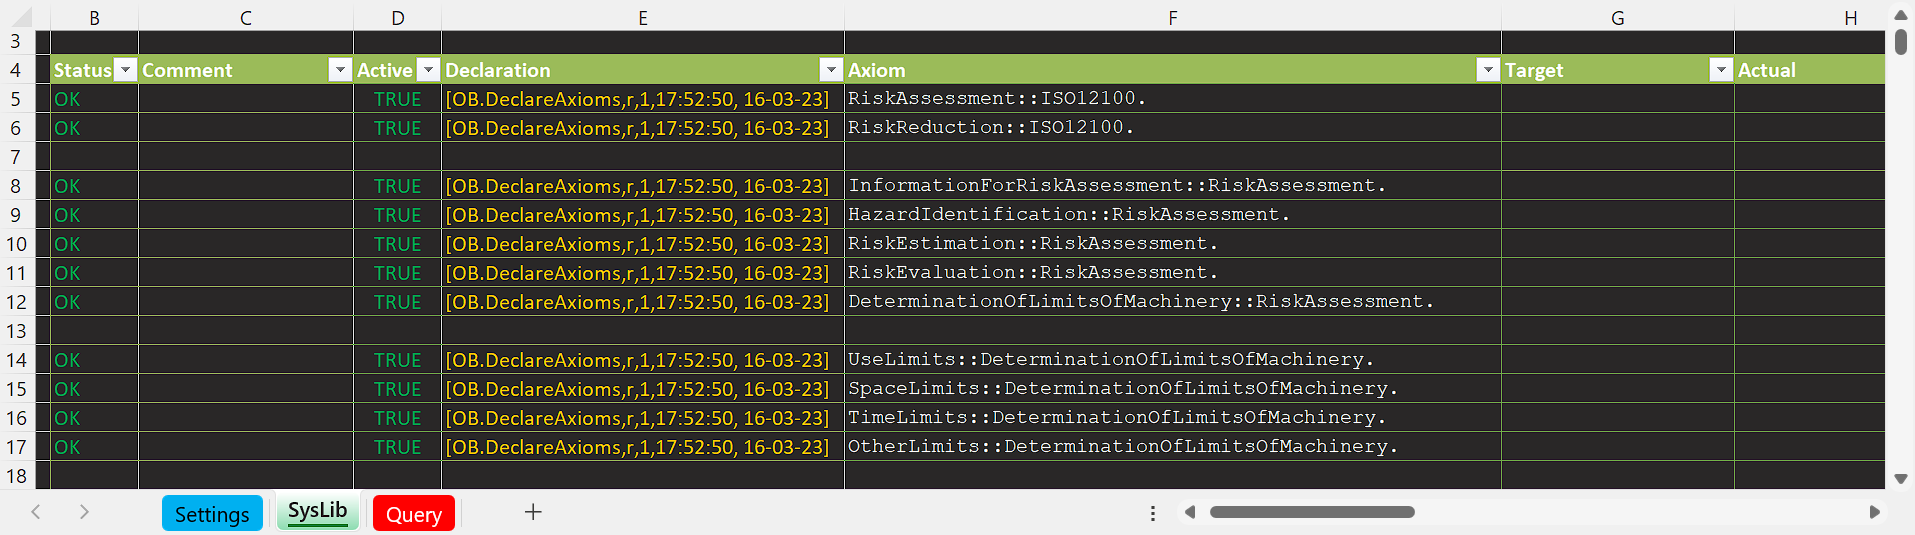
\includegraphics[width=\textwidth, height=150pt]{img/OSX_Class.png}

\bigskip\bigskip \adjustimage{width=\textwidth, height=150pt, center, caption={Class sub-class structure in OntoStudio-X}, label={fig9}, nofloat=figure, vspace=\bigskipamount}{img/OSX_Class.png}
	\chapter{Implementation} \label{implementation}

\bigskip \bigskip 

The implementation of a knowledge graph for industrial risk assessment provides a structured approach to risk management. Querying the model for a specific use case and specific implementation scenario can be beneficial for the workflow of present day risk assessment. Discussed below are a few of such scenarios which are divided into three categories according to the use cases they might serve:

\begin{enumerate}
    \item Access general information
    \item Implementation of the knowledge graph in risk assessment
    \item Specific use case
\end{enumerate}

\section{Access general information}
Querying the model allows users to retrieve specific information on the ISO 12100 safety standard in a structured manner, which is particularly beneficial for new engineers during risk assessment. To access general information, the model can be extremely beneficial for two important reasons:

\begin{enumerate}
    \item Easy access to information
    \item Time saving access to information
\end{enumerate}

Discussed below are a few use cases from the perspective of the benefits that a new engineer can enjoy while using the knowledge graph over traditional approach.

\subsection{Easy access to information}
The knowledge model contains a vast amount of information and expertise which can also be enriched. By querying the model, a new engineer can gain access to a wealth of knowledge from previous risk assessment. It can prove to be a consistent source of information to make informed decisions. The knowledge graph could help the engineer to take decisions relying on two consistent sources of information - the expert's knowledge and the safety standard. Let's start with a very basic example that the engineer wants to learn about a machine according to the ISO 12100 standard. The following relations gives the corresponding information about a machine.
\begin{itemize}
    \item hasPhaseOfMachineLifeCycle - Gives all the phases of a machine's lifecycle.
    \item safetyDependentOn - Gives information about dependency of safety features.
    \item hasPart - Components of a machine.
    \item hasFeature - Gives all the features in general a machine possess.
    \item hasState - The possible states of a machine.
\end{itemize}

The following screenshot shows the query page on Machine:

% \bigskip\bigskip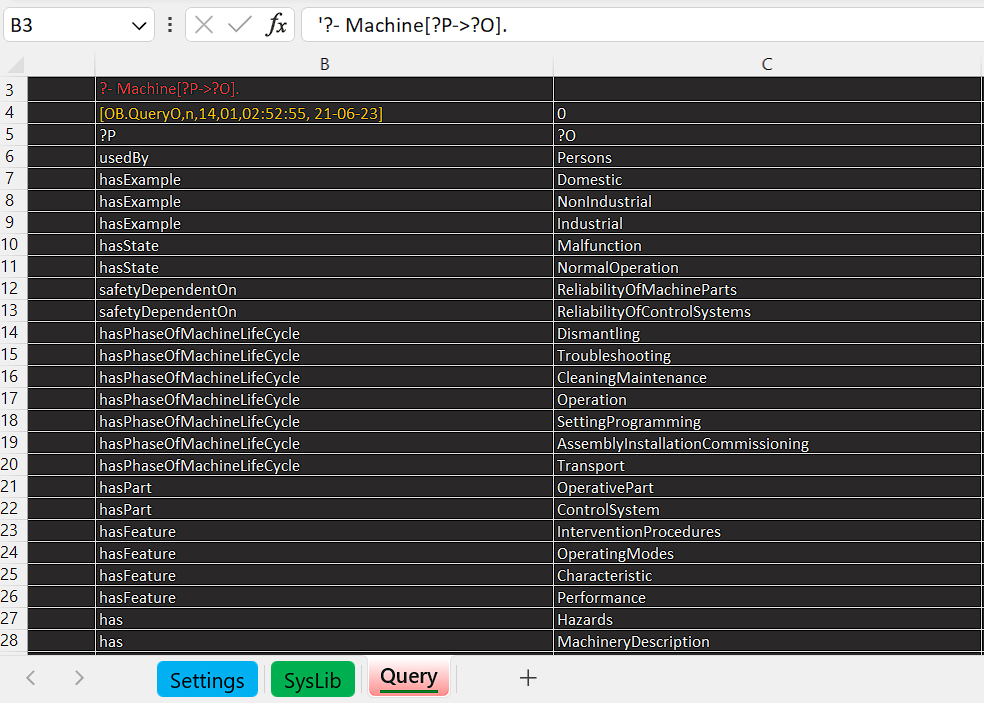
\includegraphics[width=\textwidth]{img/Machine.png}

\bigskip\bigskip \adjustimage{width=\textwidth, center, caption={Query on the concept Machine}, label={fig10}, nofloat=figure, vspace=\bigskipamount}{img/Machine.png}

\paragraph{} From the data it can be seen that one of the states of the machine could be Malfunction. A query on Malfunction can give more information as below:

% \bigskip\bigskip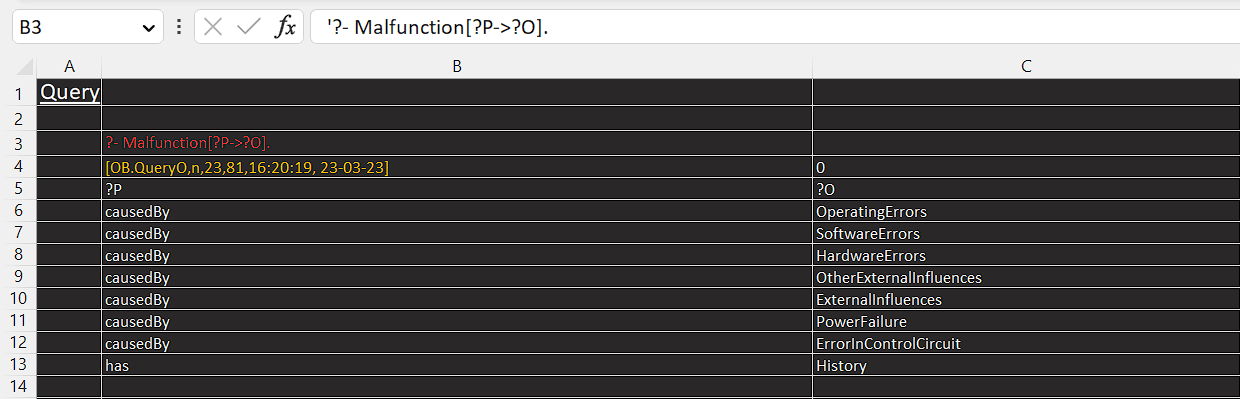
\includegraphics[width=\textwidth]{img/Malfunction.png}

\bigskip\bigskip \adjustimage{width=\textwidth, center, caption={Query on Machine state Malfunction}, label={fig11}, nofloat=figure, vspace=\bigskipamount}{img/Malfunction.png}

\bigskip\bigskip \adjustimage{width=\textwidth, center, caption={Graph visualisation of Machine state Malfunction}, label={fig11}, nofloat=figure, vspace=\bigskipamount}{img/malfunction_graph.png}

\paragraph{} It could be noted, that due to the connected nature of a knowledge graph, a Malfunction also shows up when there is a query for Hazards. Since a Malfunction is also a Hazard.

% \bigskip\bigskip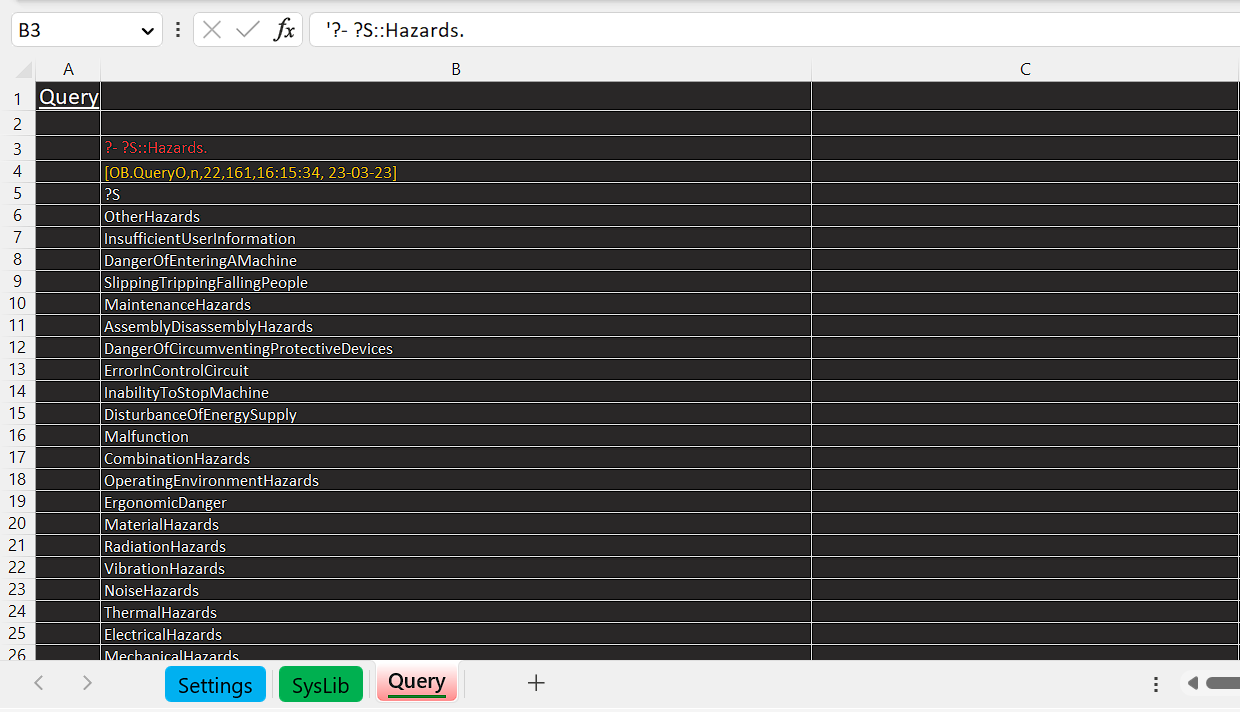
\includegraphics[width=\textwidth]{img/Hazards.png}

\bigskip\bigskip \adjustimage{width=\textwidth, center, caption={Query for the class Hazard}, label={fig12}, nofloat=figure, vspace=\bigskipamount}{img/Hazards.png}

\paragraph{} Another example can be taken here, for example a machine needs risk assessment. A simple query on RiskAssessment can give information about the three-step method (according to the ISO 12100) in a structured manner.

% \bigskip\bigskip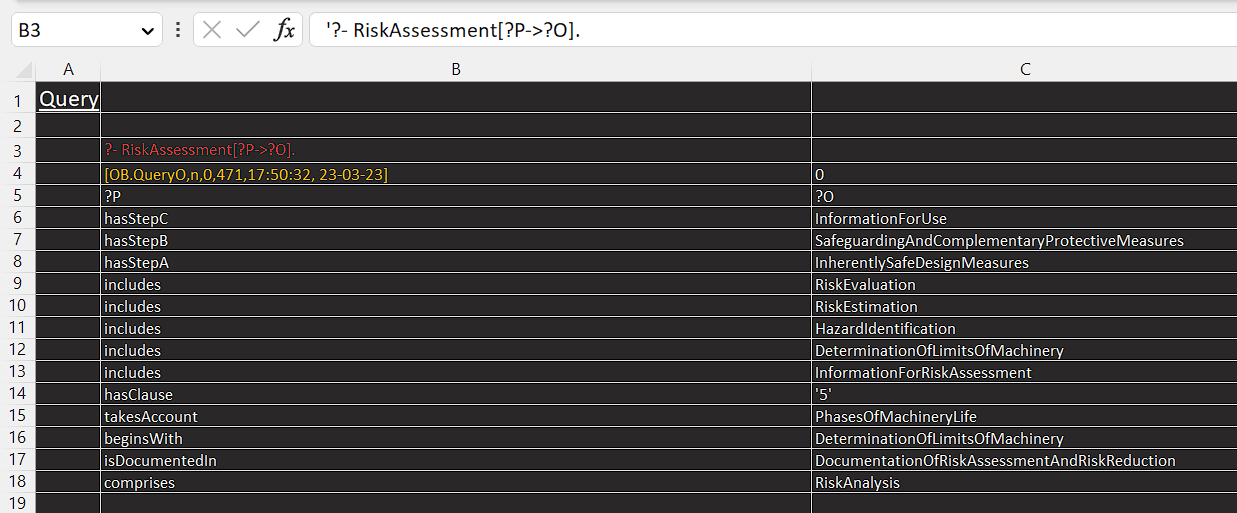
\includegraphics[width=\textwidth]{img/RiskAssessment.png}

\bigskip\bigskip \adjustimage{width=\textwidth, center, caption={Query on the concept RiskAssessment for a machine}, label={fig13}, nofloat=figure, vspace=\bigskipamount}{img/RiskAssessment.png}

\paragraph{} Each of the step here can be further queried for more information. One thing to note here, the hasClause relation shows the clause number to refer to the safety standard. For example a query on the third step, InformationForUse would give the following result:

% \bigskip\bigskip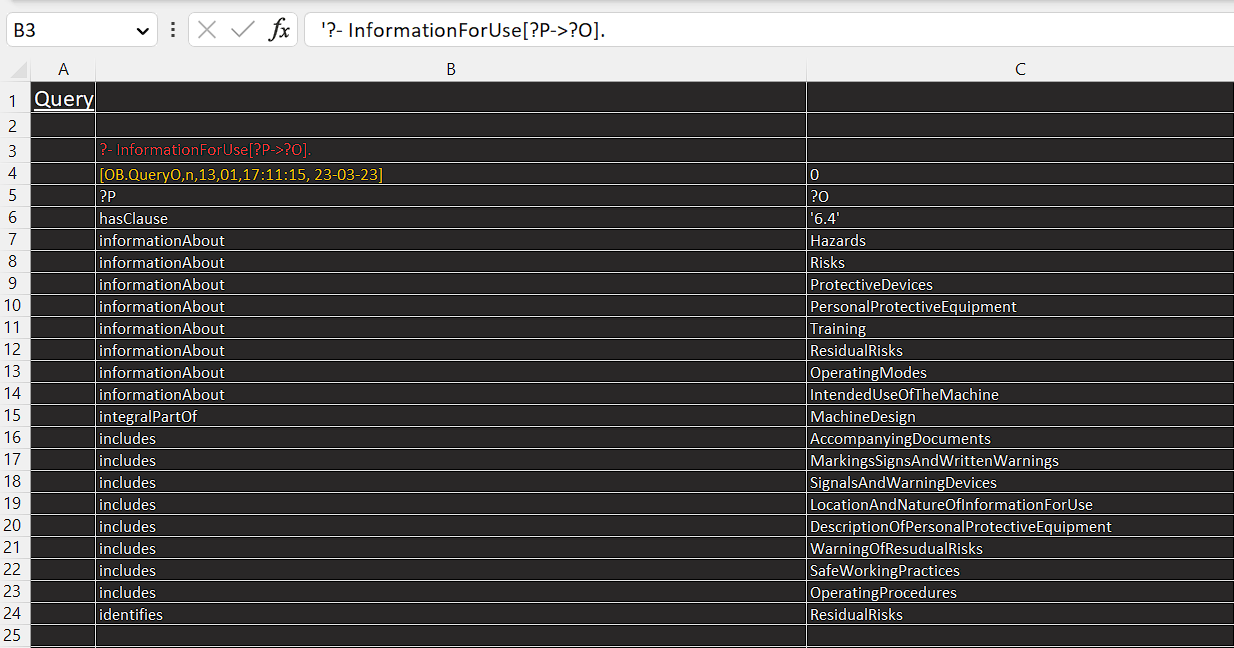
\includegraphics[width=\textwidth]{img/InformationForUse.png}

\bigskip\bigskip \adjustimage{width=\textwidth, center, caption={Query on the third step of risk assessment InformationForUse}, label={fig14}, nofloat=figure, vspace=\bigskipamount}{img/InformationForUse.png}

\paragraph{} Overall, the knowledge graph can be a useful tool for organizing and understanding complex information in a structured and intuitive way.

\subsection{Time-saving access to information}

\paragraph{} Querying a knowledge model can save a significant amount of time compared to conducting extensive research or seeking out advice from multiple experts. With the right query, a new engineer can quickly find relevant information and insights that can inform their decision-making process. It also cuts out the painstaking process of going through every line of a safety standard before every project of risk assessment. For example while working on a machinery, if the engineer wants to quickly learn about the Guards which comes under Inherently Safe Design Measures of the ISO 12100, can easily be done by querying the model. Otherwise, the engineer would have to go through the entire text written in the document to figure out each type of guard and their corresponding requirements which is an important data for risk assessment.

% \bigskip\bigskip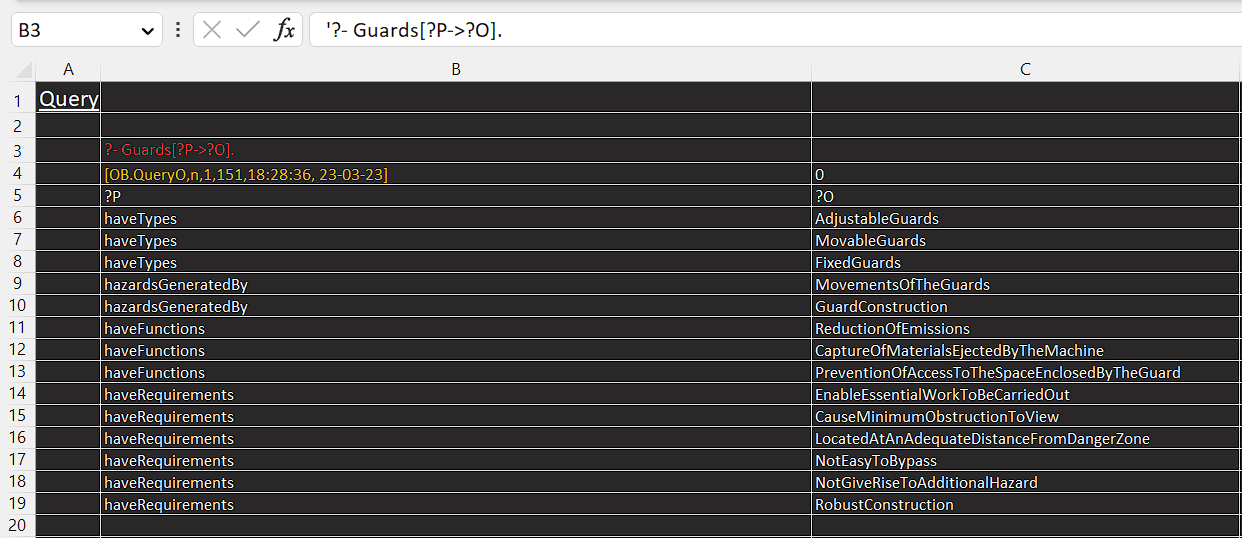
\includegraphics[width=\textwidth]{img/Guards.png}

\bigskip\bigskip \adjustimage{width=\textwidth, center, caption={Query on the concept Guards}, label={fig15}, nofloat=figure, vspace=\bigskipamount}{img/Guards.png}

The relations shown in the image are discussed below:

\begin{itemize}
    \item haveTypes - This relation gives all the types of the component.
    \item hazardsGeneratedBy - This relation gives the reason for the hazards.
    \item haveFunctions - This relation gives the functions of the component.
    \item haveRequirements - This relation gives the testing requirements of components according to ISO 12100.
\end{itemize}

The relations are pretty straightforward and from the query it is clear that there are three different types of guards. The functions of guards are displayed along with the cause of hazards from the guards. The general requirements for guards are also displayed. But if needed, specific requirements for a specific guard type can also be queried easily. For example, if the requirements for adjustable guards are needed, a quick query can give the data as below.

% \bigskip\bigskip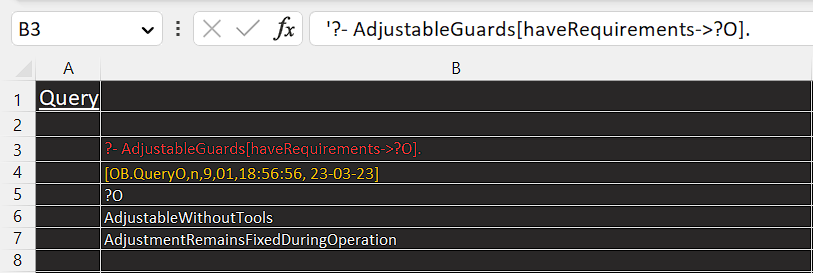
\includegraphics[width=\textwidth]{img/AdjustableGuards.png}

\bigskip\bigskip \adjustimage{width=\textwidth, center, caption={Query on the requirements for AdjustableGuards}, label={fig16}, nofloat=figure, vspace=\bigskipamount}{img/AdjustableGuards.png}

\paragraph{} A lot of other queries can be made which could be helpful in accessing general information from the knowledge graph.

\section{Implementation of the knowledge graph in risk assessment}
A knowledge graph can be a powerful tool that could be implemented in the current risk assessment process to identify and mitigate risks more effectively. This can be understood by a simple example. Suppose a new risk assessment on a Laser is to be performed. A query on the model can give information about the hazards that the laser may possess.

% \bigskip\bigskip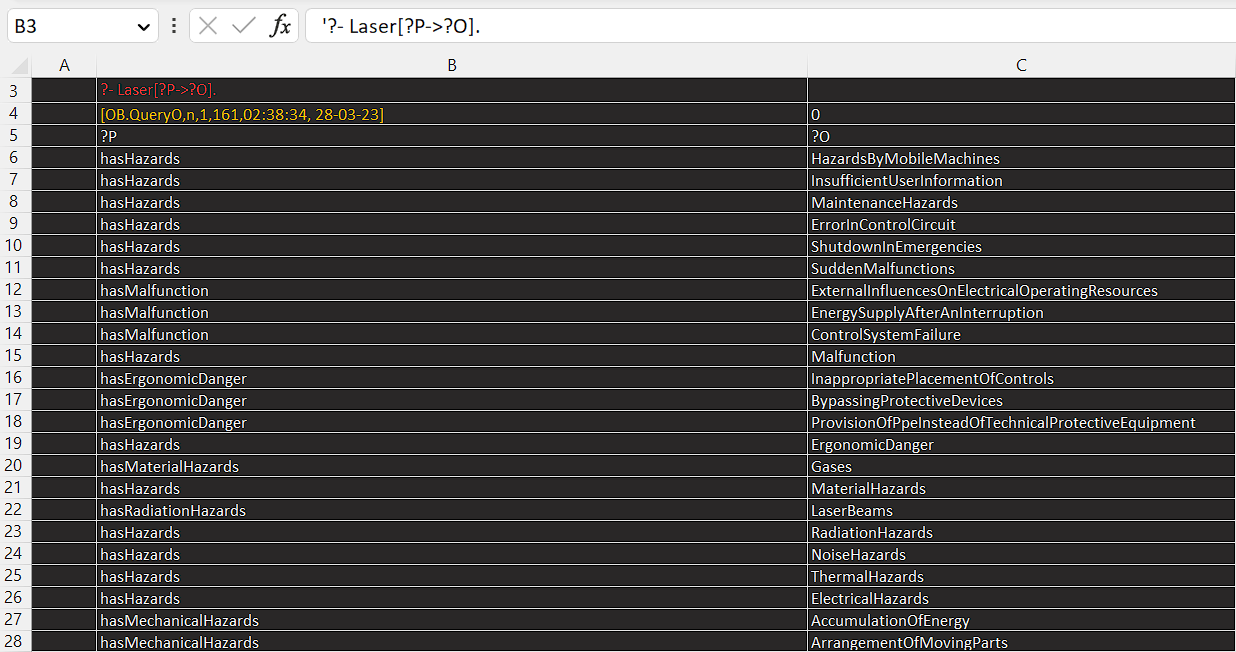
\includegraphics[width=\textwidth]{img/Laser.png}

\bigskip\bigskip \adjustimage{width=\textwidth, center, caption={Query on a machine Laser}, label={fig17}, nofloat=figure, vspace=\bigskipamount}{img/Laser.png}

Now that all the hazards of a laser are shown, it is required to mitigate the risks. For that more information is required for each hazard. Selecting one hazard at a time, for example, going with the Noise Hazard, query on the model can give the following information.

% \bigskip\bigskip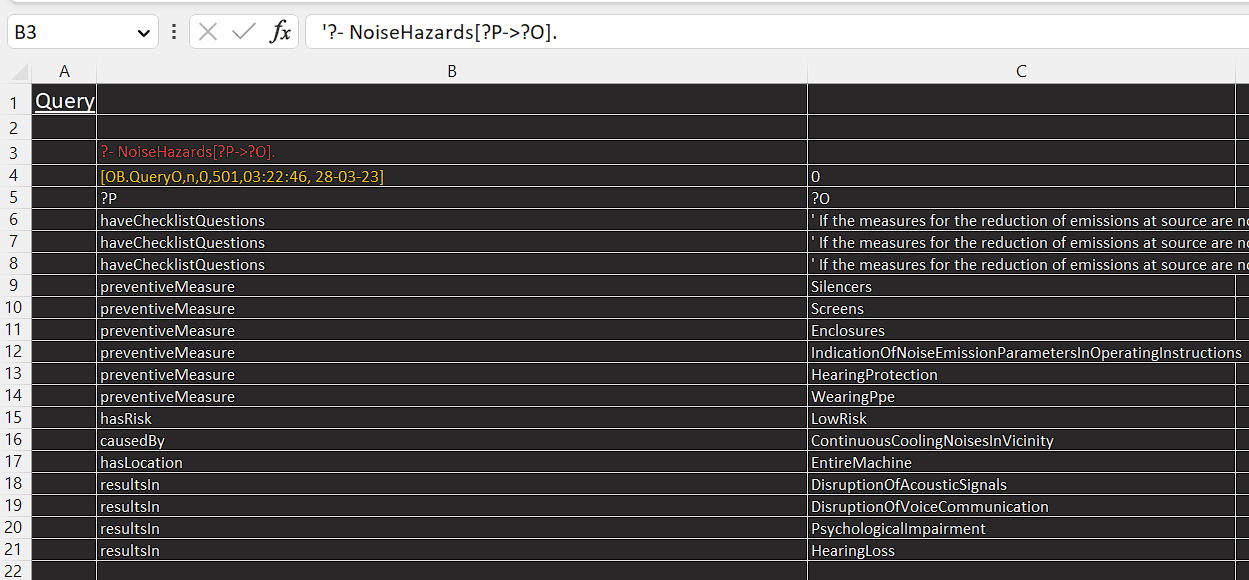
\includegraphics[width=\textwidth]{img/NoiseHazards.png}

\bigskip\bigskip \adjustimage{width=\textwidth, center, caption={Query on a hazard NoiseHazards from Laser}, label={fig18}, nofloat=figure, vspace=\bigskipamount}{img/NoiseHazards.png}

\begin{itemize}
    \item haveChecklistQuestions - This relation gives the checklist questions that need to be answered per hazard according to the ISO 12100. The safety standards mentioned as reference can be further queried to gain more information about them. For now, it only shows a brief title of the standard, but can further be expanded to allocate more data.
    \item preventiveMeasure - This relation gives the protection equipments and preventions required against the hazard. 
    \item hasRisk - Shows the risk rating of the hazard on a scale of high, medium or low.
    \item causedBy - This relation gives the possible reason of occurrence of the hazard.
    \item hasLocation - This relation gives the possible location of occurrence of the hazard on the machine.
    \item resultsIn - This relation gives the possible outcome of the hazard if it is not mitigated properly.
\end{itemize}

\bigskip\bigskip \adjustimage{width=\textwidth, center, caption={Graph visualisation of NoiseHazards from Laser}, label={fig18}, nofloat=figure, vspace=\bigskipamount}{img/noise_hazards_graph.png}

\paragraph{} All the above data could help the engineer to quickly have a glance at the important data required for the risk assessment. Also if required the engineer can update the knowledge graph with new hazard data if needed, and this information could be re-used in future risk assessment. Hence, the model could retain the expert's knowledge in a structured manner. At least that part of the expert's knowledge which can be easily formalised. 

\section{Specific use case} \label{specific_use}
In industrial risk assessment, Performance Level (PL) is an important concept particularly in the context of machinery safety. PL is used to determine the level of safety performance required of a safety-related control system or safety function, and is calculated based on the level of risk reduction required to ensure an acceptable level of safety. It is often calculated in 4 levels with level D being the being the highest level of safety performance. PL is typically used in the context of machinery safety and is based on the ISO 13849-1 standard, which provides guidelines for the design of safety-related control systems for machinery. % cite ISO 13849-1

\paragraph{} The importance of PL in industrial risk assessment lies in its ability to help ensure that machinery and equipment are designed and operated in a manner that minimizes the risk of harm to workers and the environment. By conducting a risk assessment and determining the PL required for a safety function or control system, designers and operators can implement appropriate measures to achieve the required level of safety performance. For example, if a risk assessment determines that a machine presents a high risk of injury to workers, a high PL may be required for the safety function or control system responsible for mitigating that risk. This may require the use of redundant safety features, such as emergency stop buttons, and the implementation of regular testing and maintenance procedures to ensure that the safety function or control system continues to perform at the required PL. 

\paragraph{} Now with the knowledge graph in place, finding the missing information regarding the performance level indicators is a simple task, that is, to just query the model. Hypothesis 3.1 can easily be tested here by querying all the information regarding performance level. On the other hand, hypothesis 3.2 which is about machine-to-machine communication of the performance level for automatic mitigation of risk, can be a topic of future research which can be built on top of this work. Hence Hypothesis 3.1 can be evaluated by the following query.

% \bigskip\bigskip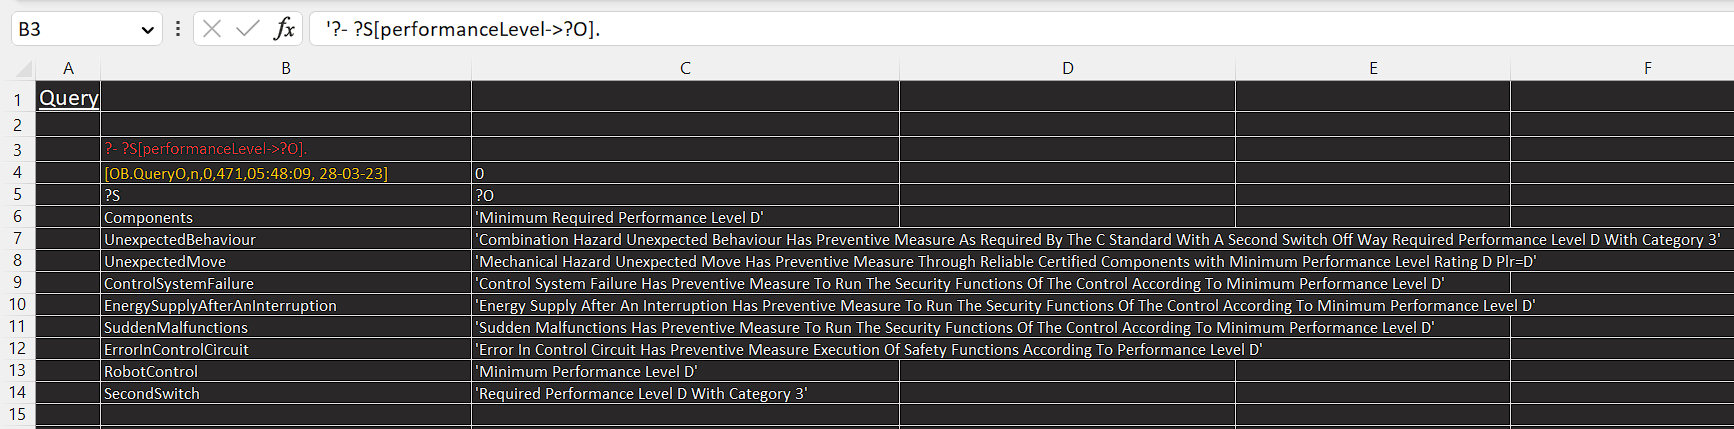
\includegraphics[width=\textwidth]{img/performanceLevel.png}

\bigskip\bigskip \adjustimage{width=\textwidth, center, caption={Query on the relation performanceLevel}, label={fig19}, nofloat=figure, vspace=\bigskipamount}{img/performanceLevel.png}

Another implementation of the knowledge graph for a very specific use case can be to search for the reference standards that are required for certain cases. This comes handy as the engineer don't need to search for the reference standard by reading through the whole document but can easily find the use cases where the reference standards are referred. A field search cannot work in this case because the reference standards are not always tagged with some keyword in the standard. Also further query on the reference standard gives a brief title of the standard which can further be expanded to accommodate the complete standard. The following query on reference standards can be cited as an example.

\bigskip \adjustimage{width=\textwidth, center, caption={Query on the relation referenceStandards}, label={fig20}, nofloat=figure, vspace=\bigskipamount}{img/referenceStandards.png}

\bigskip Alternately, if the engineer wants to find out about a particular standard 'EN ISO 13849-2' and in which cases it is referred to, the following query on the knowledge graph can suffice the purpose. This would be really helpful when the knowledge model have multiple standards. In that case searching manually for the use case of a particular reference standard would involve a lot of work.  

% \bigskip\bigskip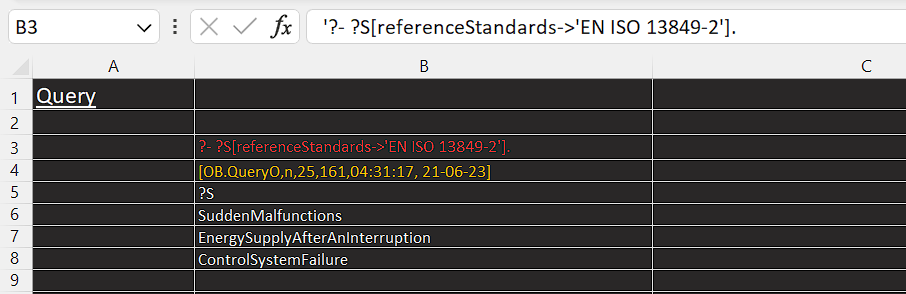
\includegraphics[width=\textwidth]{img/referenceStandards13849-2.png}

\bigskip \adjustimage{width=\textwidth, center, caption={Query on a particular reference standard}, label={fig20}, nofloat=figure, vspace=\bigskipamount}{img/referenceStandards13849-2.png}


	\chapter{Validation} \label{validation}

\bigskip \bigskip

Validation of a knowledge graph refers to the process of verifying the accuracy, completeness, and consistency of the data contained within the graph. A knowledge graph is a complex network of interrelated data points, and it is important to ensure that the data is reliable and consistent to ensure that the knowledge graph can be used effectively. Validation of a knowledge graph is particularly important in applications such as risk assessment, where inaccurate data can have significant consequences in terms of safety. For example, if the knowledge graph used to access a particular machine lacks a certain hazard in its hazard pool, or if the checklist of a certain hazard misses certain point, then the risk stays unmitigated which could be catastrophic. Validation can also be an ongoing process from the perspective of a risk assessment. As machines are evolving, standards are updating, the knowledge graph needs to be updated to incorporate all the new hazards and preventive measures that comes up with time. Thus, ongoing validation is also important to ensure that the knowledge graph remains accurate and up-to-date as new data becomes available.

\paragraph{} For this thesis, validation is mainly restricted to face validity of the knowledge graph and validation against an expert. This is inspired from the two step validation as mentioned in \cite{sim} which suggests that a model should have high face validity and good quality of output. These are divided into two separate sections (\ref{face_validity} and \ref{expert_validity}). Apart from this, the completeness of the knowledge model can be checked by re-creating a complete TRF (checklist) of the standard by querying the model and getting this TRF checked by an expert. But due to shortage in time it was not possible to get the complete TRF checked. However, the hasClause relation is used in the face validity section which can be checked with the standard to see that all the clauses have been included in the knowledge model with some depth for the respective clauses. Thus, completeness is mostly self-validated. 

\section{Face validity} \label{face_validity}
Face validity is the type of validity that refers to whether the results from the model built appears reasonable when the model is used and that the model does what it is supposed to do. Face validity makes sure that there are no clear mistakes in the model structure, whether the concepts and relations are correctly converted to SPO triples and that the model gives predictable output when queried. While these tests are mostly subjective or implemented through apparently self-validating experiments, they serve as a first sanity check for model correctness.

\paragraph{} Alongside of checking for face validity, the model is also updated to fix errors. So the approach taken was to go through the model thoroughly with the safety standard ISO 12100. This would help to examine how coherent the model is with the safety standard and that it covers the important aspects of the safety standard. It would also help to fix any missing relationships or connections or any contradictory triplets in the model. An important point should be noted here that the model is not checked for completeness but it is checked for correctness of the concepts and relations modelled.

\paragraph{} The test starts with a query for the relation hasClause. This would easily give all the important concepts present in the model that are taken from the standard and have a clause number corresponding to the standard. 

% \bigskip\bigskip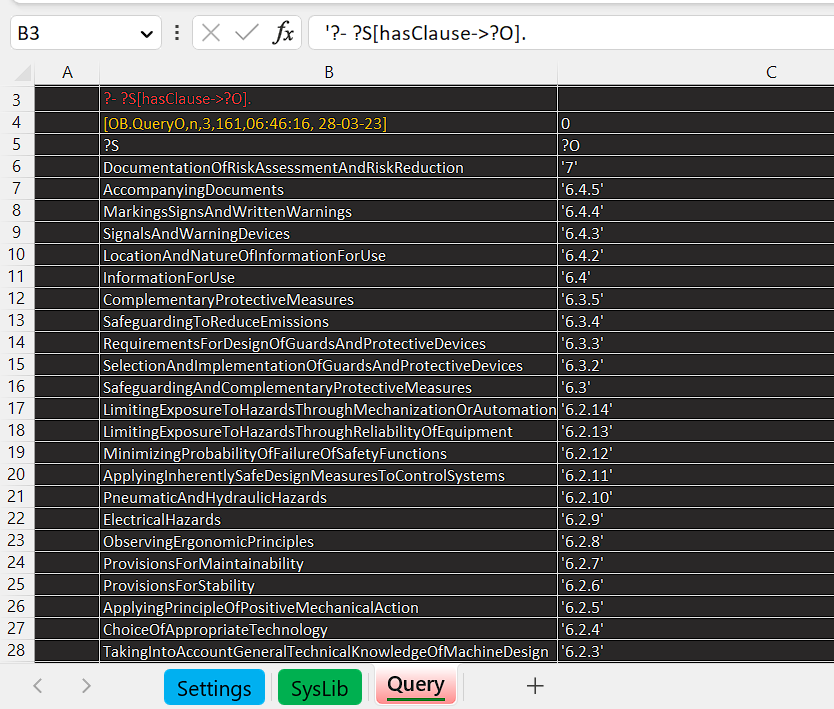
\includegraphics[width=\textwidth]{img/hasClause.png}

\bigskip\bigskip \adjustimage{width=\textwidth, center, caption={Query on the relation hasClause}, label={fig21}, nofloat=figure, vspace=\bigskipamount}{img/hasClause.png}

\paragraph{} Then each concept from clause 4 to clause 7 are queried for. Each query are continued till the depth it can go. And along with this the safety standard ISO 12100 is also referred for each clause to validate the correctness of the data. 

\paragraph{} For a few concepts, it is found that different terms are used for the same concept which does not give good results on query. Synonyms are used throughout the standard and since the knowledge graph is developed using a semi-automated approach, these synonyms are copied in the model as well. For example, the term machine and machinery means the same concept machine. But they were two different concepts in the knowledge graph. This gives dual result when there is a query related to machine. So, these synonyms are replaced with an uniform concept name throughout the model, for example "Machine" in this case. A few other similar occurrences of synonyms of other concepts are found as well and are replaced accordingly.

\section{Validation against an expert} \label{expert_validity}
Expert validation of a knowledge graph for industrial risk assessment is an important step in ensuring its accuracy and reliability. But it may not always be an easy task to achieve. There are several reasons that could make the task of validating the knowledge graph against an expert a challenging one.

\paragraph{} The knowledge graph is complex, with many concepts and relationships between them. Experts may need to spend significant time and effort understanding the knowledge graph if they were to go through each relations. Also, a semantic model is highly subjective with a lot of modelling possibilities. So it is nearly impossible for the domain expert to go through each relation and come up with a quantitative review. For this reason, face validity was performed. 

\paragraph{} Depending on the tools and technologies used to build the knowledge graph, experts may need to have some technical expertise to evaluate it effectively. And it is not always the case that an expert of machinery safety can understand how OntoBroker works or what is a knowledge model in general and how the input data is processed. This can be a barrier or maybe overwhelming for an expert to evaluate the knowledge graph in the first place.

\paragraph{} Also experts may have limited time available to review the knowledge graph, especially if they have other responsibilities or projects to manage. This can make it difficult to provide detailed feedback and suggestions for improvement. For this reason, the validation should be planned well so that it is easy for the expert to give a quantifiable review of the model as well as it is the fastest way of validation possible.

\paragraph{} The relation haveChecklistQuestions would provide the questions that can be used in a checklist for risk assessment. A few sections are selected and for each of them the checklist questions are queried from the model. These questions are then transferred to a TRF (Test Report Form). An example of the checklist questions for Noise Hazard is shown below. 

% \bigskip\bigskip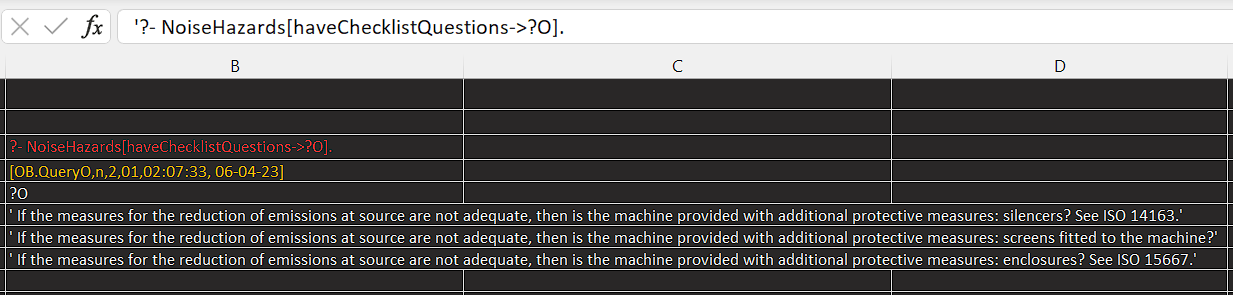
\includegraphics[width=\textwidth]{img/NoiseHazards_Checklist.png}

 \bigskip\bigskip \adjustimage{width=\textwidth, center, caption={Query for the checklist questions for noise hazard}, label={fig22}, nofloat=figure, vspace=\bigskipamount}{img/NoiseHazards_Checklist.png}

\paragraph{} The questions are separated per section and the corresponding clause number are also mentioned which would make them easier to refer from the ISO 12100. The clause number can easily be queried with the relation hasClause. The TRF is a document that is used everyday by an expert to perform risk assessment, so the format of the document is well known to him/her. Also it is very easy to transfer the checklist questions queried from the knowledge graph to a TRF. It would involve just copy and paste of the data. So now the expert can easily look at questions for the corresponding sections of the TRF and comment on its correctness. This is the easiest and the fastest way in which the output from the model could be validated by an expert. It would also save time and effort of an expert. An example page of the TRF output from the knowledge graph is shown below in Figure \ref{fig23}.

% \bigskip\bigskip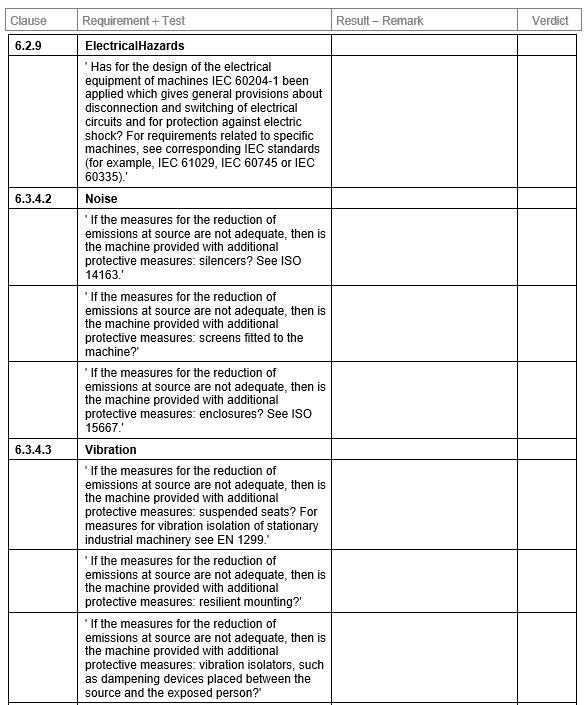
\includegraphics[width=\textwidth]{img/TRFoutput_from_KG.png}

\bigskip \adjustimage{width=\textwidth, center, caption={Checklist questions in TRF format}, label={fig23}, nofloat=figure, vspace=\bigskipamount}{img/TRFoutput_from_KG_2.png}

\paragraph{} The evaluation sheet is divided into two sections, namely, correctness of the checklist from the knowledge model and usefulness of the knowledge model. Validation would be incomplete without quantifiable results as they provide a clear and objective way to measure the performance or accuracy of the model. The expert is provided with an evaluation sheet along with the TRF output. The expert can then check for correctness of the TRF output for the selected clauses. The expert can rate between a score of 1 to 4 for each of the selected clause. The filled evaluation sheet is attached below in Figure \ref{fig24}.

\bigskip \adjustimage{width=\textwidth, center, caption={Evaluation sheet for the correctness of the knowledge model}, label={fig24}, nofloat=figure, vspace=\bigskipamount}{img/checklist_evaluation.png}

\paragraph{} The clauses where the knowledge model is said to not fully reach expectations are due to referencing of another standard. The external standard is referenced only for the first point but they need to be referenced for all points. The input data for these checklist questions comes from a previous risk assessment where the references were not such. But with this review from the expert, the knowledge model is also updated to include the reference. 

\paragraph{} After validating the correctness, it is also important to review the structure of the model for its usefulness in risk assessment. The usefulness of the knowledge model is evaluated after a brief explanation of the implementation of the knowledge graph to two experts. The points for usefulness of the model is based on the implementation of the model in current risk assessment which is described in chapter \ref{implementation} of this thesis. The implementation of the knowledge graph is demonstrated to the experts and they could rate between a score of 1 to 4 for each use case. Similar to the rating used to evaluate the correctness of the checklist generated from the model. The final scores are averaged in the filled evaluation sheet which is attached below in Figure \ref{fig25}.

% \bigskip\bigskip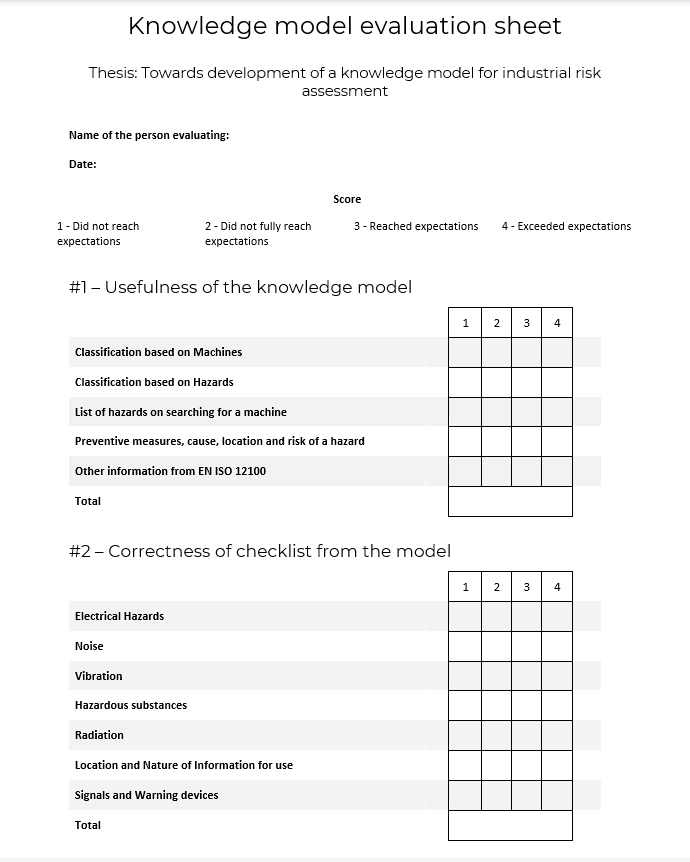
\includegraphics[width=\textwidth]{img/evaluation_sheet.png}

\bigskip\bigskip \adjustimage{width=\textwidth, center, caption={Evaluation sheet for the usefulness of the knowledge model}, label={fig25}, nofloat=figure, vspace=\bigskipamount}{img/checklist_review.png}
	\chapter{Future Applications} \label{applications}

\bigskip \bigskip 

The main benefit of this work is towards making a faster, cheaper and safer industrial risk assessment.   
\begin{itemize}
	\item \textbf{Faster}: The risk assessments can be reused and hence machines can be tested faster.
	\item \textbf{Cheaper}: Less time required for assessment and less manual work required means lower costs involved.
	\item \textbf{Safer}: Safe assessment only with the relevant requirements and information per project. This can help to identify hazard and mitigate them easily.
\end{itemize}

With knowledge being digitized, the expert's interpretation of a standard can be structured into a knowledge model. This in turn would help in future risk assessments. The fuzzy requirements from standards can be interpreted correctly as the data from the standard now is not only just text but converted into a knowledge graph with nodes and edges. The structured knowledge from domain expert can help in refining the requirements better. With the information being captured by a knowledge model and is described in a machine-understandable way, it paves a path for an artificially intelligent (“smart”) software. The smart software could be able to reason about this model. This can incur new facts (or requirements) to be derived automatically from the knowledge model, or existing facts (or requirements) can be verified. 

\paragraph{} With a semantic model in place, machine to machine communication of risk assessment for risk assessment can be made possible. New hazards can be identified and can be mitigated automatically. 

\section{Implementation in the tool for risk assessment}

Apart from the implementations and uses as mentioned in chapter \ref{implementation}, the knowledge graph can also be used in the current risk assessment process in other ways. To harness the full capabilities of a knowledge graph, it can be integrated with a risk assessment software just like mCom ONE. This can be done by developing an integration layer that allows the software application to access and query the knowledge graph. This may involve developing APIs, data connectors, or other integration mechanisms. This implementation is not done in this thesis but can be considered as an extension to this project into an already existing tool. This integration can be beneficial in the following ways:

\begin{enumerate}
    \item Data Integration: The knowledge graph is used to integrate data from different sources and formats into a single coherent model. This can be useful when the application mCom ONE needs to access data from different sources, such as a combination of structured and unstructured data, and across different domains. By integrating data of a knowledge graph, the application can have a more complete understanding of the data, which can enable more sophisticated analysis, risk assessment and decision-making. 
    \item Semantic Search: A knowledge graph can be used to improve the accuracy and relevance of search results from the application. The knowledge graph can enable more precise and relevant search results, by understanding the relationships between entities and concepts. This can help users quickly find relevant information and insights, which can support more effective risk management.
    \item Personalized Recommendations: The knowledge graph can enable more accurate and personalized recommendations, based on the relationships between entities and concepts. This can support more effective risk management, by tailoring recommendations to the specific needs and requirements of individual users. For example, while evaluating a particular hazard, similar related hazard that can also co-exist can pop-up as recommendation to be considered alongside.
    \item Improved Collaboration and Communication: The knowledge graph can enable more effective collaboration and communication between different stakeholders involved in risk management. By providing a shared understanding of the data and its relationships, the knowledge graph can support more efficient and effective decision-making processes.
\end{enumerate}

Looking at the above benefits, existing features in mCom ONE can be improved as well as new features can be added. The help option can be improved. A chat-bot can be developed to give quick information about the safety standard. A recommender system can be developed for the search bar which can give related results when searching for a hazard. The hazard pool can be automatically updated with data from the knowledge graph. Hazards and control measures can be better connected. The checklist based audit can be improved where safety standards are not always well defined and requirements which are sometimes fuzzy. With semantic technologies, like the knowledge graph in place, software applications for industrial risk assessment like mCom ONE can be made better. Since, a knowledge graph have the potential to significantly improve the accuracy, efficiency, and effectiveness of software systems and applications, and enable more advanced data processing, analysis, and decision-making capabilities \cite{text2kg}.

\section{Future development} \label{future_use}
The future applications of a knowledge model in industrial risk assessments are vast and varied, as technological advances and data-driven approaches continue to shape the field of industrial risk management. The knowledge model can be integrated with various other technologies. Here are some potential future applications:
\begin{itemize}
    \item \textbf{Integration with IoT:} The integration of knowledge models with Internet of Things (IoT) devices can enable real-time risk monitoring, as well as automated risk assessment and management. IoT devices such as sensors, cameras, and wearables can collect data on safety conditions, equipment status, and worker behavior. This data can be fed into the knowledge model, which can then analyze the input to identify potential safety hazards and suggest risk mitigation strategies. This can also happen in real-time with an actuator in place to mitigate the risk or an alarm to alert of a possible threat. For example, in a machine if a sensor (for example a camera) detects that the measures for the reduction of radiation at source are not adequate and the machine is not provided with adequate protective measures, such as use of guards or filtering according to 6.3.4.5 of ISO 12100, then an alarm for non-compliance can be put up in real-time and the risk of radiation emission can be mitigated. Thus integration of IoT devices is actually a head-start towards machine-to-machine communication in risk assessment.
    \item \textbf{Use of Artificial Intelligence:} The use of machine learning and artificial intelligence algorithms in knowledge models can improve risk assessment accuracy, identify complex patterns and relationships, and enable predictive maintenance and optimization. AI algorithms can help the model to understand human behaviour and patterns with better accuracy. The incorporation of human factors into knowledge models can enable a more comprehensive understanding of risks, as well as the development of human-centric risk management strategies that address the interaction between humans and machines. For example, with an AI algorithm in place which is being fed on several recent accident reports, it can detect a pattern of the most common risk that is causing accidents and the knowledge model can be queried for the risk and the corresponding preventive measures which can then be checked in the first place for future risk assessments. Thus such integration of AI algorithms with the knowledge model can suggest for the root causes of recent incidents and corrective actions to prevent similar incidents in the future. 
    \item \textbf{Simulation for risk assessment:} Simulation can be an useful addition to the knowledge model for risk assessment of complex systems. According to Zio \cite{ZIO2018176}, simulation can be a fundamental tool for knowledge retrieval. By running a set of simulations with different initial configurations of system design and operation parameters, the different system state can be evaluated along with the corresponding safety conditions. These safe states can then be recorded into the knowledge model. Thus, simulation can be a probable source for knowledge elicitation apart from safety standards and previous risk assessments. And the knowledge model can be enriched with a wide range of system information and safe conditions for several configurations.
\end{itemize}

Integrating these technologies with the knowledge model for risk assessments can provide more comprehensive and effective safety solutions, thereby, reducing the risk of incidents and improving safety culture in industrial settings. These improvements can enable a more efficient, and effective approach to industrial risk management, leading to better safety, reliability, and productivity in industrial settings. 

\section{Machine-to-machine communication} \label{m2m}
Machine-to-machine communication (M2M) of a knowledge model in industrial risk assessments can enable real-time and automated risk management processes as discussed by Bunte \cite{Bunte2020}. A similar work is done by Salim Khan et al. \cite{Khan2022}, the paper proposes an IoT-based system that uses Raspberry Pi and sensors to collect real-time data from machines, such as voltage, current, gas value and temperature. The data is then processed by a machine learning model that compares it with training data and generates statistical graphs of machine performance. The paper claims that the proposed system can help to monitor and analyze the machines in an industrial environment and predict the possibility of upcoming risks. 

\subsection{Advantages} 
Machine-to-machine communication of a knowledge model for industrial risk assessment has several advantages. One of the main benefits is that it enables more efficient and effective risk assessment processes. By automating the collection and analysis of safety data, M2M communication can reduce the time and effort required for risk assessment and help identify potential hazards more quickly and accurately. Additionally, M2M communication can enable real-time monitoring of safety conditions, allowing for rapid responses to emerging risks. This can be particularly important in dynamic environments such as manufacturing facilities, where conditions can change quickly and unpredictably.

\paragraph{} Another advantage of M2M communication is that it can help ensure that updated safety standards are consistently applied across an organization. By providing a shared knowledge model of safety standards that can be accessed and utilized by all relevant parties, M2M communication can help minimize inconsistencies in safety assessments and ensure that safety protocols are followed consistently across different departments and locations. This can be especially beneficial for large organizations with multiple locations and teams that may have different interpretations of safety standards. By having a shared knowledge model, which is being updated in real-time, all parties involved in industrial risk assessment can work from the same set of guidelines, reducing the risk of errors or oversights due to misunderstandings or misinterpretations of safety standards.

\paragraph{} By facilitating real-time data exchange between machines and systems, M2M communication can enable the collection and analysis of large amounts of data related to machine performance and maintenance needs. This data can then be used to identify patterns and trends, and to predict when machines are likely to require maintenance or replacement. With this predictive maintenance approach, potential machine failures can be detected and addressed, before they result in downtime or hazards. This helps to reduce the likelihood of accidents and injuries in the workplace, and can also result in significant cost savings by reducing the need for unplanned maintenance or equipment replacement. Overall, the use of M2M communication for predictive maintenance can improve both safety and efficiency in industrial settings.

\paragraph{} As new risks are identified, they can be added to the knowledge model and shared with relevant parties and machines in real-time, allowing for a more comprehensive and up-to-date understanding of potential risks. This can also enable more proactive risk management by allowing for the identification and mitigation of potential risks before they become major issues. Additionally, by using a shared semantic knowledge model, all machines can have a standardized and consistent understanding of the risks, leading to better communication and collaboration in automated risk management.

\paragraph{} The above potential future applications of the semantic model capable of machine-to-machine communication for risk assessment can easily be understood with a simple real life scenario. For example, if a machine working for over a decade has an accident, the hazard can be shared with similar machines that are prone to such accident. Also, the manufacturer can change some requirements to mitigate the hazard over the semantic web. By sharing the updated risks and hazards in a shared semantic knowledge model through M2M communication, other similar machines or equipment can benefit from the knowledge and take necessary precautions to prevent accidents. This can help to ensure that the hazard is not repeated in the future and that preventive measures are taken to mitigate the risk. Additionally, manufacturers can use this information to improve their designs and prevent similar accidents from happening in the future. The relevant safety standards can also be updated accordingly. Ultimately, this can save lives, reduce injuries, and minimize damage to property and equipment. The work presented in this master thesis would serve as the preliminaries of such use cases and this work can be extended towards machine communication of hazards.

\subsection{Limitations}
While M2M communication has many advantages and probable use cases, it has has some limitations which can be worked on. One limitation is that it requires a reliable and secure network to function properly. If the network infrastructure is not reliable, there may be issues with data transmission, which can result in delays, errors, or loss of data. This can impact the effectiveness of risk assessment processes. Another limitation for M2M communication can be the compatibility of the different systems used. If the systems are not compatible, it can be challenging to establish M2M communication between them, and this can hinder the effectiveness of risk assessments.

Also as identified by several works like in \cite{Kadena2017} and \cite{TUNA2017142} security risks are a major threat for M2M communication. Protection against unauthorized access and modification of safety parameters in the knowledge model must be prevented. All data exchanged between machines should be encrypted to prevent unauthorized interception. This can be achieved using various encryption protocols, such as Transport Layer Security (TLS) or Secure Sockets Layer (SSL). To detect and prevent potential security breaches, intrusion detection systems can be implemented. These systems can monitor network traffic and alert administrators of any suspicious activity or attempts at unauthorized access. A knowledge model for safety standards on cyber-physical systems can be employed here for continuous monitoring. IEC 62443 can be used according to the work of Halenar et al. \cite{Halenar2023} which proposes an architecture of the cybernetic systems in a smart
factory with a focus on communication security. Securing such cyber-physical system and M2M communications against cyber threats especially for safety projects of TIC industry can be an interesting and important topic for future research.

\paragraph{} M2M communication may require a significant investment in terms of infrastructure, and training. Organizations may need to invest in new technologies and equipment, and need to train their staff on how to use these new systems effectively. The initial investment and ongoing maintenance costs can be significant, and organizations need to weigh these costs against the potential benefits of M2M communication for risk assessment.
	\chapter{Challenges and limitations} \label{challenges}

\bigskip \bigskip 

While there are many potential benefits to using a knowledge graph for industrial risk assessment, there are also several challenges and limitations that should be considered. These challenges are discussed in this chapter. The challenges can primarily segregated into two sections.
\begin{enumerate}
    \item Challenges faced in the development process
    \item Potential challenges in the implementation
\end{enumerate}

\section{Challenges faced in the development process}

In this section, the challenges that came across the development process of the knowledge graph is discussed. The part of development which requires further research and development is the section for input data \ref{gather_relevant_data}. The quality and completeness of the data used to populate the knowledge graph are critical factors that can impact the effectiveness of risk assessment. If the data is incomplete, inconsistent, or inaccurate, it can lead to incorrect assessments. An improper risk assessment can be dangerous. Therefore, it is essential to establish an assurance process of the quality of input data to ensure that the data used to populate the knowledge graph is accurate, consistent, and complete and avoid GIGO (garbage in, garbage out) as much as possible. However, it must be done in the most automated way possible due to the huge volume of text data as input. 

\paragraph{} The development of an ontology that accurately represents the concepts and relationships from the safety standard should be made efficient and accurate. According to F. N. Al-Aswadi et al \cite{al-aswadi_chan_gan_2019} fully automatic construction of ontologies from text is still a major challenge. The semi-automated approach used to generate SPO triples from text for this thesis work is also manual labour intensive. Most of the effort required towards development of the knowledge graph went towards perfecting the SPO triples manually. Therefore, further development of ontology creation techniques that require less human intervention still remains a challenge and is an interesting area to study.

\paragraph{} Safety standards are sometimes not well defined. Developing safety standards requires a general agreement among stakeholders, which can be difficult to achieve. Different stakeholders may have different priorities, perspectives, and interests, which can make it challenging to develop standards that are widely accepted and effective. Safety standards thus may vary across different cultures and regions, reflecting differences in values, and priorities. This can make it challenging to develop a knowledge graph which is consistent, uniform and accurate for the safety standards. It requires general understanding of the standards and the new risks and hazards to develop a knowledge graph which could again be a big challenge towards automatic development of knowledge graphs from standards.

\paragraph{} If the knowledge graph is built on a large scale for a TIC organisation, there would be massive amount of data to build the model. It means digitisation of a large number of safety standards and test documents. Construction and maintenance of such quantity of data requires a dedicated department which could be expensive. It requires investment in data input, ontology development, computing resources, and software development. Dealing with large and complex datasets may require investment in high-performance computing infrastructure and specialized software tools to support the development and maintenance of the knowledge graph. Also updating the knowledge graph is significantly important as risks are constantly evolving. As technology advances, new safety issues may arise that are not covered by existing standards. This can create gaps in risk assessments, which can leave unmitigated risks. This makes it an important as well as a challenging task to update the knowledge graph efficiently. So developing the Machine-to-Machine communication of risks \ref{m2m}, which is a challenging task in itself is also required to be worked on simultaneously.

\section{Potential challenges in the implementation}
In this section, the challenges that can hinder the implementation of a knowledge model in industrial risk assessments is discussed. There are several reasons that can keep it far from achieving industrial risk assessments using knowledge models. The success depends heavily on user acceptance and adoption which is also the main challenge to overcome. Users here are the person who would perform the risk assessment using the new technology.

\paragraph{} Users may be resistant to change and may prefer to use existing tools and processes. This can be particularly challenging when introducing a new technology like a knowledge graph, which may require changes to existing workflows and processes. Users may not be aware of the benefits of a knowledge graph or how it can be used to support decision-making. This can impact user acceptance, as users may not see the value in using a knowledge graph. To address this challenge, it is important to communicate the benefits of using a knowledge graph and to engage users in the development and implementation of the technology. Providing user training and support can also help to raise awareness of the benefits of using a knowledge graph and can also help to ease the transition to the new technology.

\paragraph{} Knowledge graphs can be complex, particularly when dealing with large and diverse datasets. This complexity can make it challenging for users to navigate and understand the information presented in the knowledge graph, which can impact user acceptance. Knowledge graphs sometimes may require technical knowledge to use effectively. Users may need to understand the underlying ontology and the relationships between concepts in the domain. This can be a barrier to adoption for users who do not have the required technical knowledge or training. To address this challenge, it is important to design an intuitive user interface with which the user can interact easily and can get the desired information quickly, without requiring a deep understanding of the underlying technology. 

\paragraph{} Finally, organizational stand point is the most important aspect to embrace a change. The culture and organizational structure of an organization can impact user acceptance directly. Some organizations may be more open to adopting new technologies, while others may be more resistant to change. Orthodox organizations may fear actual implementation of new technologies especially if they are disruptive to existing processes or require significant investment. This can pose as a major challenge. To address this challenge, it may be necessary to build a culture of innovation and openness to change within the organization. This can involve engaging with stakeholders at all levels of the organization, communicating the benefits of using a new technology which can make risk assessments more efficient. It is required to start small with the implementation and test their effectiveness and impact on existing workflows. A change can bring a competitive advantage to stay ahead of the curve and develop products and services that meet the needs of a changing world. 
        \chapter{Conclusion} \label{conclusion}

\bigskip \bigskip The thesis is concluded by discussing the main contributions and an overall summary of the work done. The contribution contains the results and conclusions for each research question that were discussed in \ref{rq}.

\section{Contributions}

The thesis covers the following research questions.

\rqformat{\textbf{RQ 1:} How can industrial safety assessments be made faster and efficient?}

\paragraph{} This is a broad question and can further be divided into the further questions which follows. But as a general answer, industrial safety assessment can be made faster and efficient by changing the current workflow. Currently, risk assessment is mostly done manually and is primarily based on an expert's interpretation of safety standards. Also safety standards are not always well-defined and the requirements are sometimes vague. This makes the current process of risk assessment slow and inefficient if it is done manually and only at an expert's discretion. However, the process can be made faster and efficient by digitizing the workflow of current risk assessment. This thesis, mainly focuses on the digitization of knowledge captured from the experts and from safety standards. 

\rqformat{\textbf{RQ 2:} How can knowledge from experts and standards be captured for re-use?}

\paragraph{} To address this question, a knowledge model is developed for industrial risk assessment. The complete methodology is discussed in Chapter \ref{method}. The two sources of input data of this model are the safety standard ISO 12100 and an expert's knowledge from a previous risk assessment. A semi-automated approach is adopted to extract knowledge which is described in \ref{gather_relevant_data}. An NLP based information extraction pipeline is used to extract knowledge in a structured way from general text data. But this algorithm is not always accurate, so manual work is still required for knowledge extraction. Knowledge is extracted as SPO (Subject-Predicate-Object) triples. Semantic technology like a knowledge graph is considered to use for this work since the input data for the model is textual and can best fit the purpose. A class hierarchy structure as defined in \ref{class_hierarchy} is prepared as an outline, which helps to build the knowledge graph. The tools used to develop the knowledge graph are described in \ref{develop} along with the development process in which the SPO triples are structured into a knowledge graph. Most of the process is automated wherever possible. 

\rqformat{\textbf{RQ 3:} How to deal with the missing information regarding the performance level indicators?} 

\paragraph{} This question can be answered once the knowledge model is prepared. The solution can be found with the implementation of the knowledge model in Chapter \ref{implementation}, section \ref{specific_use}. A simple query to the model for performance level can show the minimum performance level required by a safety component to mitigate the risk. This is beneficial in risk assessment as the expert now no longer need to search the safety standard to find the required performance level, which can sometimes be difficult to find. Apart from this, Chapter \ref{implementation} also contains other use cases where the knowledge graph can benefit the current risk assessment process.

\rqformat{\textbf{RQ 3:} How can the knowledge model be validated?}

Validation is the most important part of developing the knowledge model since it is built to be used in industrial safety assessments. So in Chapter \ref{validation}, it is discussed how to ensure that the model have a high face validity and a good quality output which is also a validated by a human expert. Face validity is performed by going through the model thoroughly along with the safety standard by the process described in \ref{face_validity} and fix errors simultaneously. This serve as a first step of sanity check for the model correctness. Expert validation of the output from the model is the next important step for validation to ensure its accuracy and reliability. This is done by generating a checklist for few clauses from the knowledge graph and presenting the output in a familiar format of a TRF (Test Report Form) to the expert. This makes it easy to go through the output for the expert and it is also the fastest way of validating the knowledge graph. An evaluation sheet is also prepared with which the expert can give a quantifiable result of the knowledge model.

\section{Summary}

In conclusion, this thesis proposes the development of a knowledge model to support industrial risk assessment. The introduction begins with the motivation to work for this thesis from the perspective of a TIC (Testing, Inspection and Certification) industry. The problems that can come up while working for this thesis are also discussed along with the research questions and proposed hypotheses which are addressed in the section above. Then the background of how industrial risk assessment is performed currently is presented, which contains a brief about safety standards and the ISO 12100. The different techniques to model knowledge and how modeling of knowledge can help industrial risk assessment is also discussed. A literature review is also conducted on the works that are related to this thesis.

\paragraph{} The main part of the work contains a systematic methodology to develop the knowledge model. The scope and purpose of the model is discussed. Extracting knowledge from the safety standard and the expert is an important task which needs to be done most efficiently. Here, a semi-automated approach is discussed which is used for knowledge extraction. The concepts and relations are structured into SPO (Subject-Predicate-Object) triples by this approach. Then the knowledge graph is prepared based on a hierarchical structure of the concepts. The SPO triples is formalized with ObjectLogic and the knowledge graph is finally built with OntoBroker. After development, it is also necessary to implement the model in several use cases of risk assessment. A few implementations are discussed which can be done with the model built. Validation of the model is the most important part of building a model and it is done against an expert. A quantitative review of the output from the model ensures the accuracy and reliability of the model.

\paragraph{} After the development phase, future applications of the model is discussed. How the model can be improved and what further developments can be made for future risk assessments. An interesting concept of machine-to-machine communication is also discussed for a futuristic automated risk assessment. Finally, the challenges faced in the development process are discussed along with the challenges that can hinder the implementation of knowledge model in risk assessments.
	\begin{appendix}
		\chapter{Repository}
        \paragraph{} The repository for the working files of this thesis is uploaded to GitHub 
		\dots{}
	\end{appendix}
\end{document}
